\documentclass[a4paper,12pt]{article}

% Packages nécessaires
\usepackage[utf8]{inputenc}
\usepackage[T1]{fontenc}
\usepackage[french]{babel}
\usepackage{graphicx} % Pour inclure des images
\usepackage{caption} % Pour personnaliser les légendes
\usepackage{array} % Pour les tableaux
\usepackage{mathpazo} %police pas mal
%\usepackage{lmodern} % Police Latin Modern
\usepackage{amsmath} % Pour les formules mathématiques
\usepackage{geometry} % Pour ajuster les marges
\usepackage{fancyhdr} % Pour personnaliser les en-têtes et pieds de page
\usepackage{tikz} % Pour les images en arrière-plan
\usepackage{lipsum} % Pour générer du texte d'exemple
\geometry{top=4cm, bottom=2.5cm, left=2.5cm, right=2.5cm, headheight=2cm, headsep=1cm}
%\renewcommand{\thetable}{Tableau \arabic{table}}
\usepackage[normalem]{ulem}
\usepackage{float} % For the 'H' float option
\useunder{\uline}{\ul}{}


% Début du document
\begin{document}

% Page de titre
\begin{titlepage}
    \begin{minipage}[t]{0.4\textwidth}
        
\includegraphics[width=\textwidth]{media/logo-enit-2454399073.png} \\[1cm] % Logo de l'établissement
    \end{minipage}
    \centering
    \vspace*{2cm}
    \begin{tikzpicture}[remember picture, overlay]
        \node[opacity=0.2, anchor=south] at (current page.south) {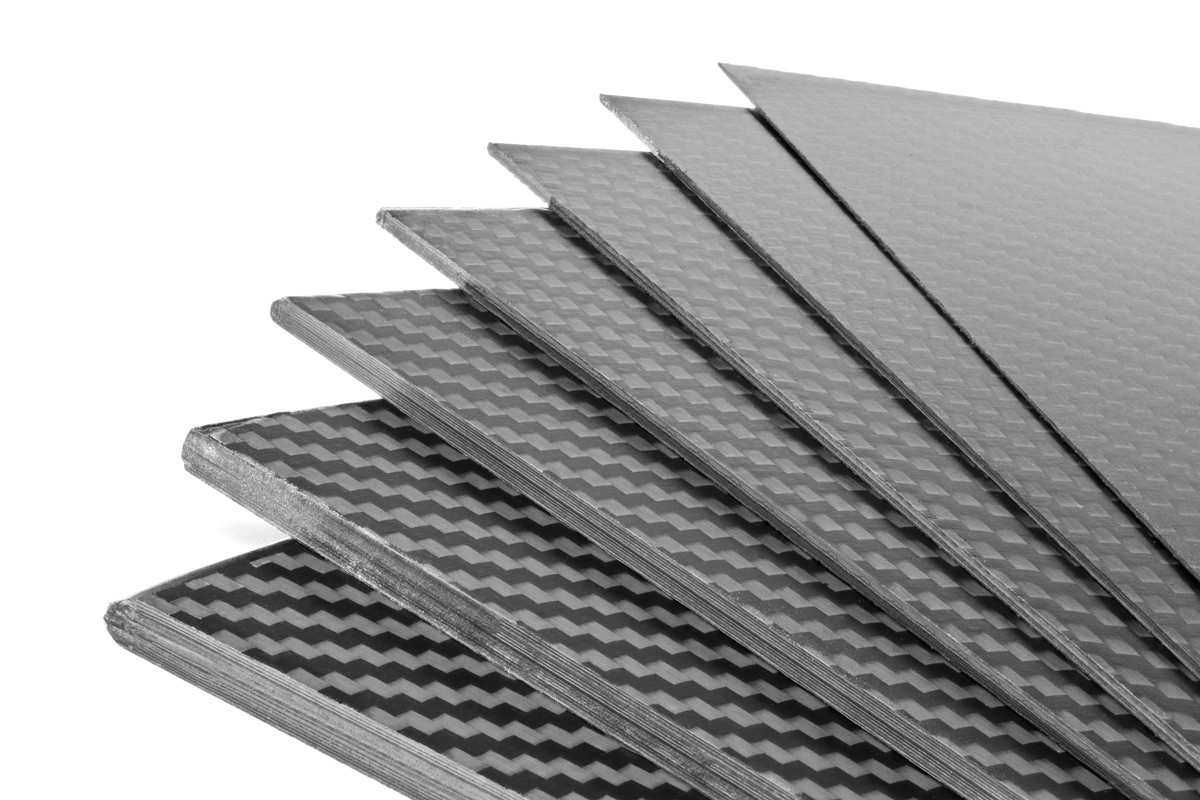
\includegraphics[width=1\paperwidth]{media/plaquecarbonne.jpg}}; % Image d'arrière-plan
    \end{tikzpicture}
    
    {\scshape \Large Rapport de TP} \\[0.5cm] % Type de document
    {\Huge \textbf{Structures composites}} \\[1.5cm] % Titre du TP
    {\large \textbf{Killian RENOU \\ William GUILBERT}} \\[0.5cm] % Noms des auteurs
    {\large \textbf{Date : 12/04/2025}} \\[0.5cm] % Date
    {\large \textbf{ENIT - École Nationale d'Ingénieurs de Tarbes}} \\[0.5cm] % Établissement
    \vfill
    {\large \textbf{Encadrant : Christian GARNIER}} % Nom de l'encadrant
\end{titlepage}


% Configuration des en-têtes et pieds de page
\pagestyle{fancy}
\fancyhf{} % Efface les en-têtes et pieds de page par défaut
\fancyhead[L]{
\includegraphics[width=3cm]{media/logo-enit-2454399073.png}} % Logo à gauche
\fancyhead[C]{\textbf{Rapport de TP Structures Composites}} % Titre au centre
\fancyhead[R]{\textbf{ Killian RENOU  \\ William GUILBERT}} % Noms à droite, l'un sous l'autre
\fancyfoot[R]{\thepage} % Numéro de page centré en pied de page
\renewcommand{\headrulewidth}{0.4pt} % Ligne noire sous l'en-tête

% Table des matières
\tableofcontents
\newpage

% Introduction
\section{Introduction}

Ce rapport présente une analyse comparative de différentes configurations de plaques soumises à un chargement mécanique, dans le cadre du cours de structures composites. L'objectif principal est d'évaluer les performances mécaniques de plaques composites asymétriques et symétriques, ainsi que d'une plaque en acier, en utilisant des outils numériques tels qu'Abaqus et une feuille de calcul dédiée.

Le contexte de cette étude s'inscrit dans la conception de structures légères et résistantes, où les matériaux composites jouent un rôle clé grâce à leur rapport résistance/poids élevé et leur capacité à être optimisés pour des applications spécifiques. Cependant, leur comportement complexe nécessite une modélisation précise et une validation rigoureuse.

Les objectifs de ce travail sont les suivants :
\begin{itemize}
	\item Définir les hypothèses nécessaires à la mise en place des modèles numériques.
	\item Comparer les résultats obtenus sous Abaqus avec ceux issus de la feuille de calcul composite.
	\item Identifier les limites des configurations initiales et proposer des optimisations pour répondre aux critères de résistance.
	\item Comparer les performances des plaques composites avec celles d'une plaque en acier.
\end{itemize}

Cette étude permettra de mieux comprendre les avantages et les inconvénients des matériaux composites par rapport aux matériaux traditionnels comme l'acier, tout en mettant en lumière les défis liés à leur dimensionnement.

% Plaque 1
\section{Plaque 4 plis sans symétrie miroir sous chargement mécanique}
\subsection{Hypothèses nécessaires à la mise en place du modèle numérique}
\begin{table}[H]
	\centering
	\renewcommand{\arraystretch}{1.2} % Augmente l'interligne des lignes du tableau
	\begin{tabular}{r p{10cm}}
		Formulation & Structure, coque 2D     \\
		\hline
		Espace de modélisation & 3D (Courbure induite par l'asymétrie de la structure soumise à de la traction)  \\
		\hline
		Géométrie   & Plaque de William (L=150mm, l=400mm), plaque de Killian (L=400mm, l=400mm)\\
		\hline
		Matériau   & Pli composite UD, Loi de comportement: linéaire élastique isotrope transverse (E\textsubscript{l} = 38 Gpa, E\textsubscript{t} = 9 Gpa, $\nu$\textsubscript{lt} = 0,32, G\textsubscript{lt} = 3,6 Gpa)\\
		\hline
		Comportement de structure   & Coque 2D composite, Lay-Up \\
		\hline
		Type d'analyse   & Statique, temps d'analyse: 1s\\
		\hline
		Cas de chargement   & \begin{tabular}[t]{@{}p{10cm}}
			Pas de conditions initiales ni de conditions aux limites \\
			Force linéique N\textsubscript{xx} (l.a: l1+l2, direction x, sens: +x (l1), -x (l2), Amplitude = 1000 N.mm\textsuperscript{-1}) , \\
			Force linéique N\textsubscript{yy} (L.a: L1+L2, direction y, sens: +y (L1), -y (L2), Amplitude = 500 N.mm\textsuperscript{-1}) , \\
			Force linéique N\textsubscript{xy} (L.a: L1+L2, direction x, sens: +x (L1), -x (L2), Amplitude = 250 N.mm\textsuperscript{-1}) , \\
			Force linéique N\textsubscript{xy} (l.a: l1+l2, direction y, sens: +y (l1), -y (l2), Amplitude = 250 N.mm\textsuperscript{-1}) , \\
		\end{tabular} \\
		\hline
		Maillage   & \begin{tabular}[t]{@{}p{10cm}}
			Famille d'éléments: coque \\
			Bibliothèque d'éléments: standard \\
			Forme d'éléments: quadrilatère \\
			Nombre de nœuds par élément: 4 (interpolation linéaire)\\
			Nombre de DDL par noeud: 5 \\
			Intégration réduite\\
			Taille d'éléments optimisée\\

		\end{tabular} \\
		\hline
		Donnée de sortie   & U, $\sigma$, $\varepsilon$, Critère de rupture \\
	\end{tabular}
	\caption{Hypothèses pour la plaque 1}
	\label{Tableau 1: Hypothèses pour la plaque 1}
\end{table}

\subsection{Mise en place du modèle numérique sous Abaqus}
Les hypothèses nous ont permis de mettre en place le modèle numérique de la plaque 1 en considérant l'empilement suivant:

\begin{table}[h!]
	\renewcommand{\arraystretch}{1.2} % Augmente l'interligne des lignes du tableau
	\centering
	\begin{tabular}{c|c|c}
		\textbf{N° pli} & \textbf{Orientation (°)} & \textbf{Epaisseur (mm)} \\
		\hline
		4         & 15              & 1,5            \\
		3          & -30              & 1            \\
		2          & -15              & 1,5           \\
		1         & 30             & 1           \\
	\end{tabular}
	\caption{Lay-up de la plaque 1 asymétrique}
	\label{tab:exemple_tableau}
\end{table}

\begin{figure}[h!]
	\centering
	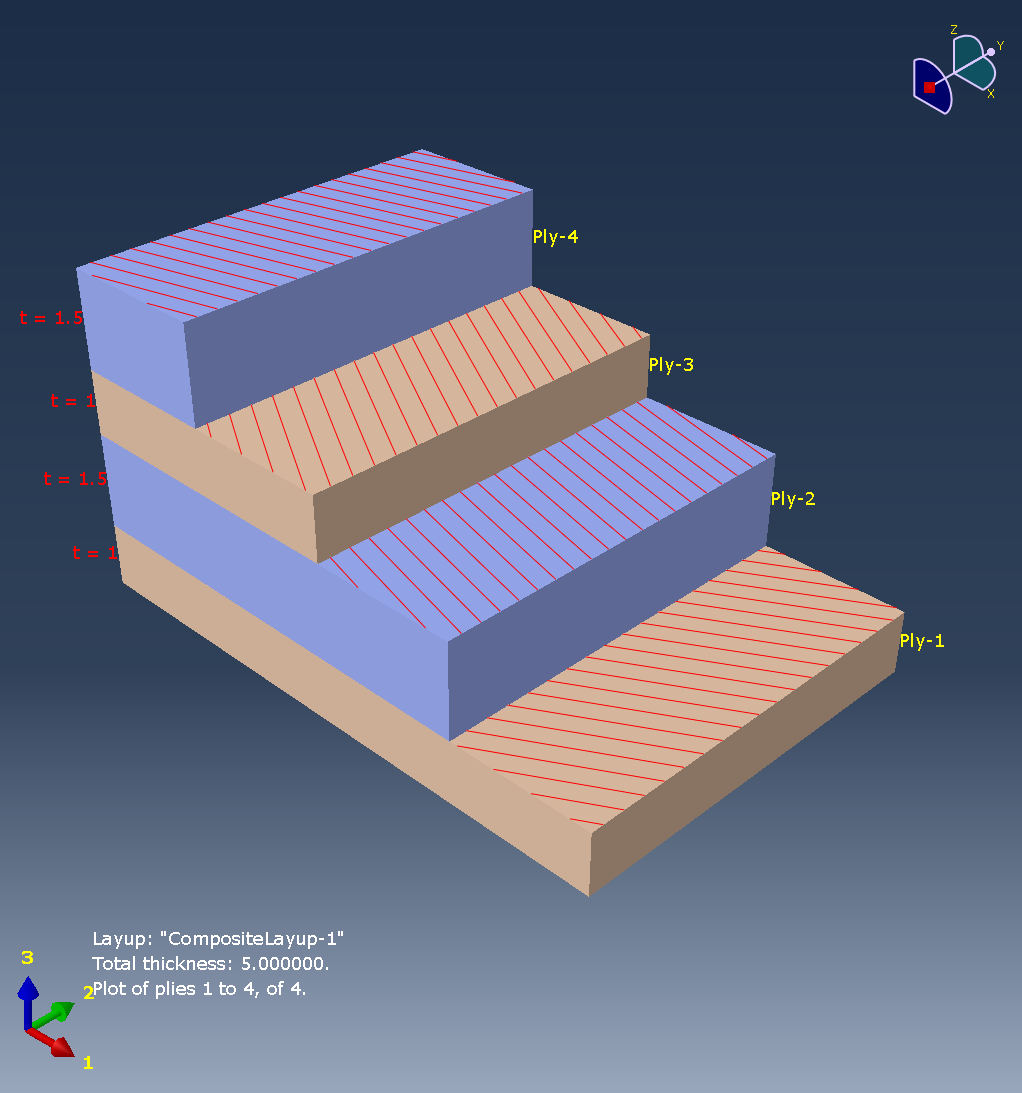
\includegraphics[width=0.5\textwidth]{media/K_P1_layout_12042025.png} % Remplacez par le chemin de votre image
	\caption{Lay-up de la plaque 1 visualisé sous Abaqus.}
	\label{fig:exemple_image}
\end{figure}

\subsection{Résultats obtenus sous Abaqus}

%résultats de la plaque 1, couche 1
\begin{figure}[h!]
	\centering
	\begin{minipage}[t][0.3\textheight]{0.495\textwidth}
		\centering
		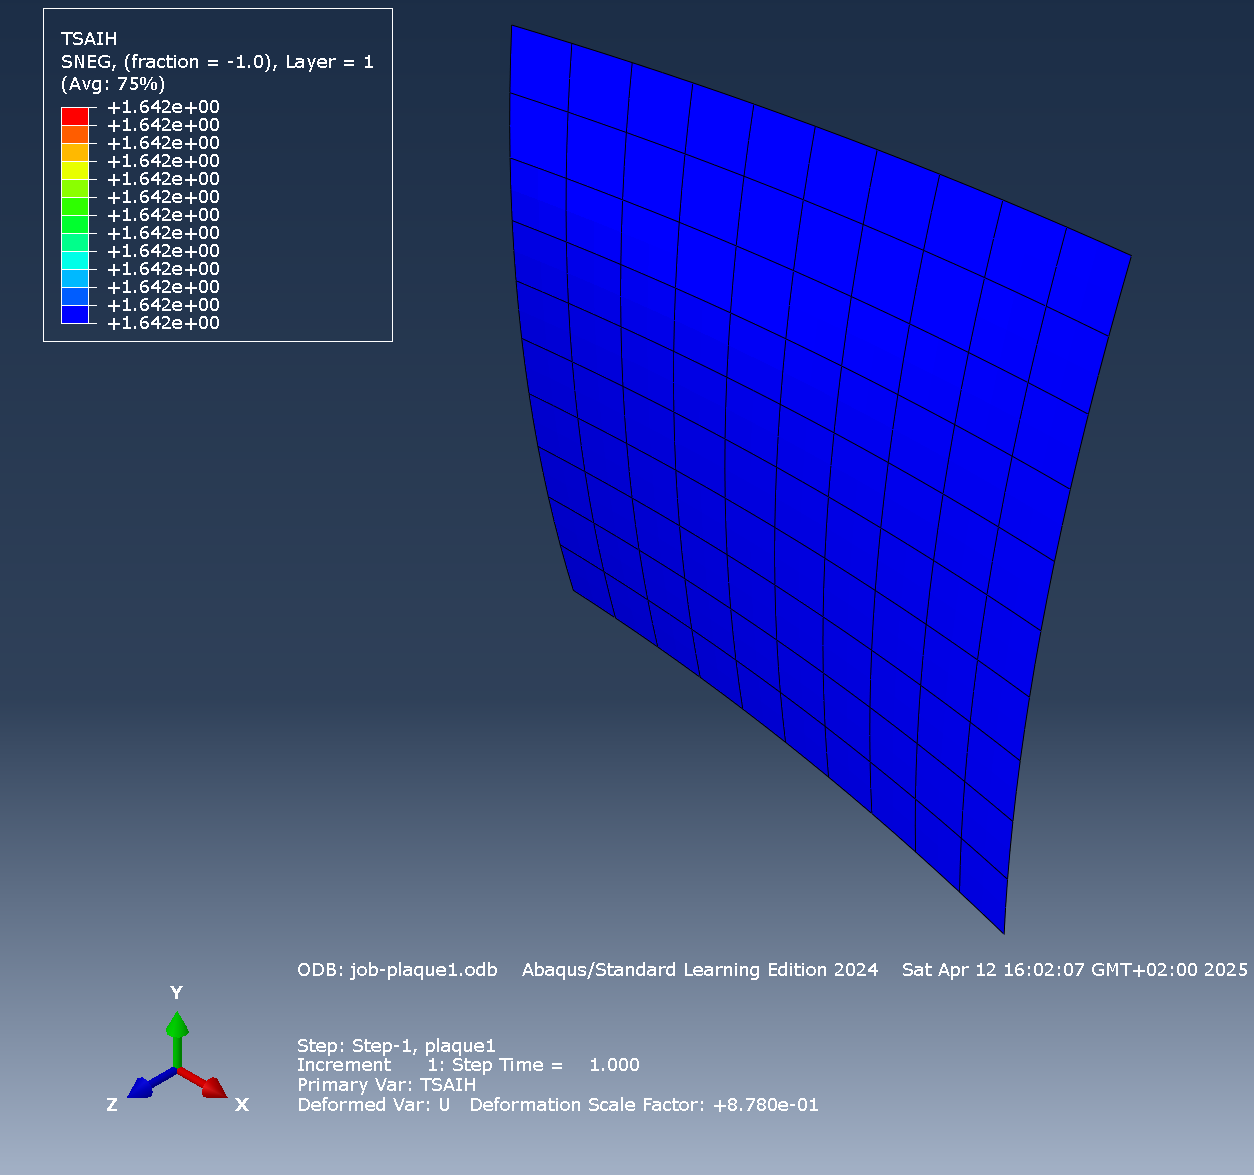
\includegraphics[width=\textwidth]{media/K_P1_L1_12042025.png} % Remplacez par le chemin de votre première image
		\caption{Couche 1, plaque carrée (Killian)}
		\label{fig:image1}
	\end{minipage}
	\hfill
	\begin{minipage}[t][0.3\textheight]{0.495\textwidth}
		\centering
		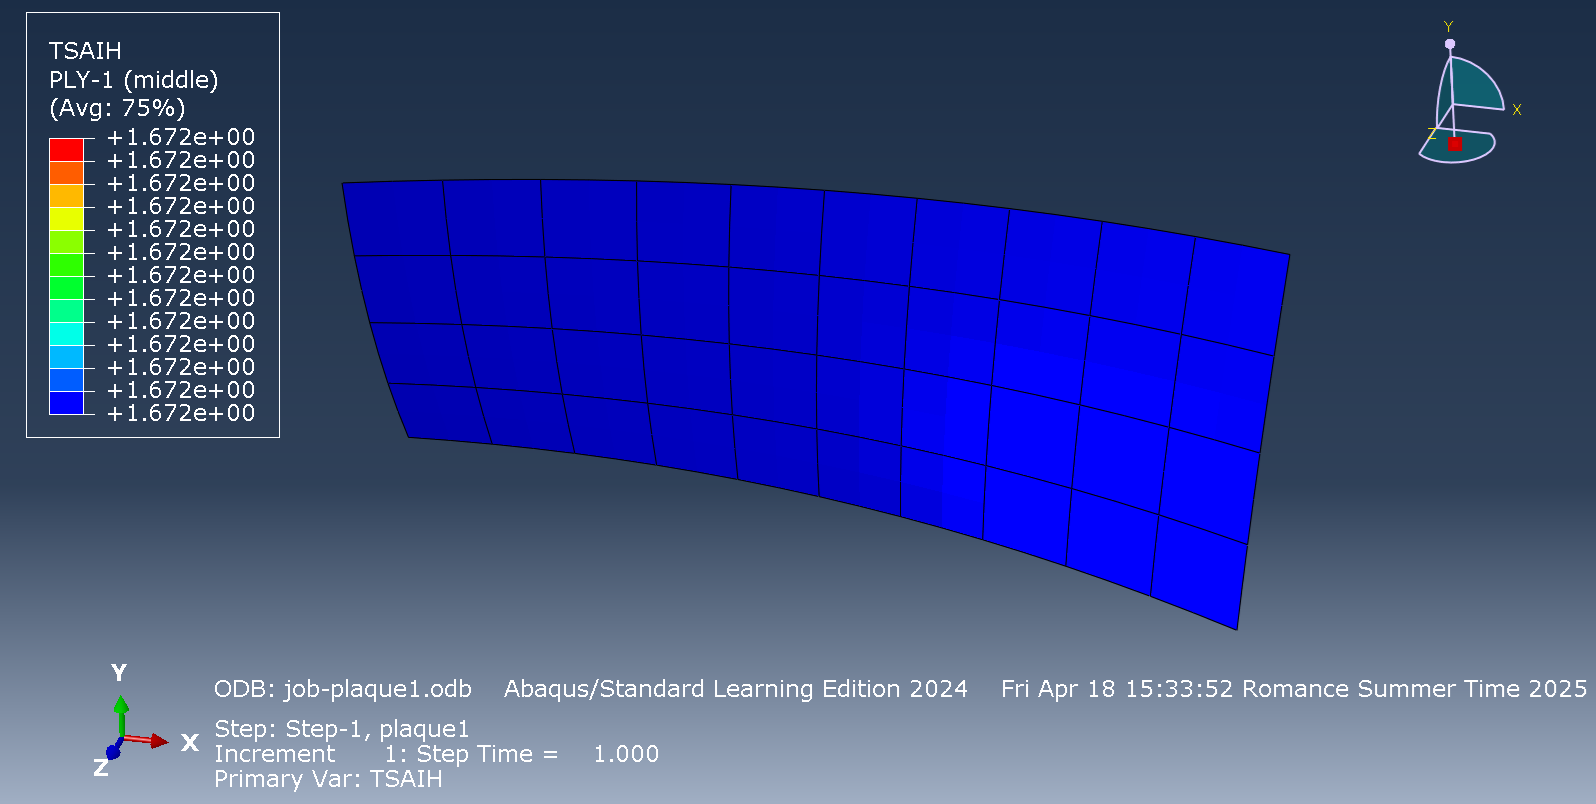
\includegraphics[width=\textwidth]{media/Couche1_.png} % Remplacez par le chemin de votre deuxième image
		\caption{Couche 1, plaque rectangle (William)}
		\label{fig:image2}
	\end{minipage}
\end{figure}

%résultats de la plaque 1, couche 2
\begin{figure}[h!]
	\centering
	\begin{minipage}[t][0.3\textheight]{0.495\textwidth}
		\centering
		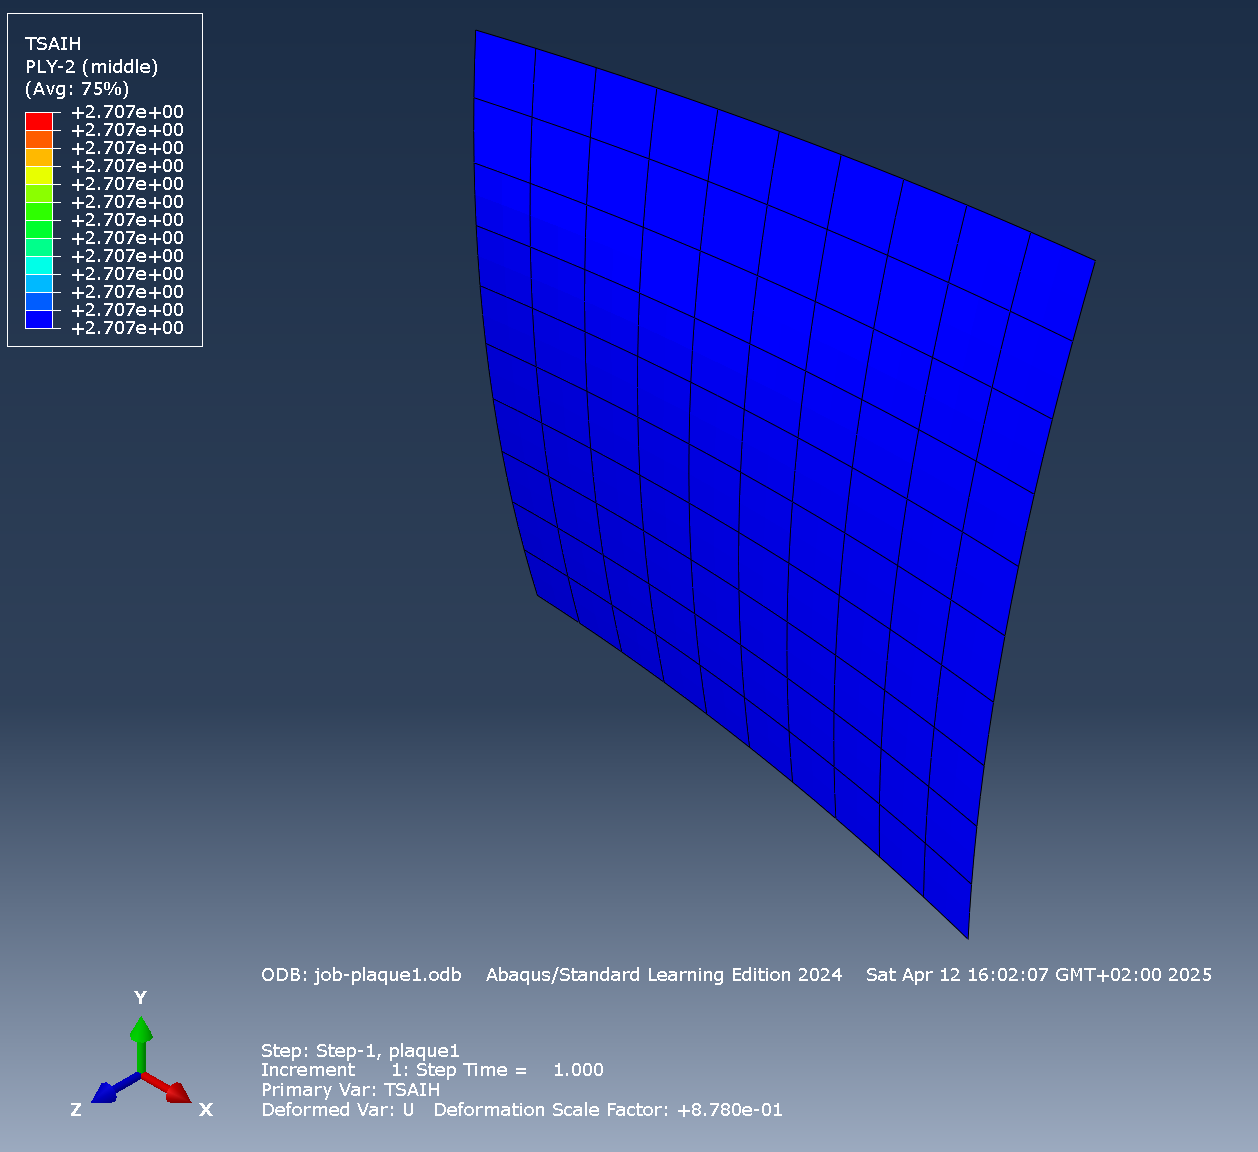
\includegraphics[width=\textwidth]{media/K_P1_L2_12042025.png} % Remplacez par le chemin de votre première image
		\caption{Couche 2, plaque carrée (Killian)}
		\label{fig:image1}
	\end{minipage}
	\hfill
	\begin{minipage}[t][0.3\textheight]{0.495\textwidth}
		\centering
		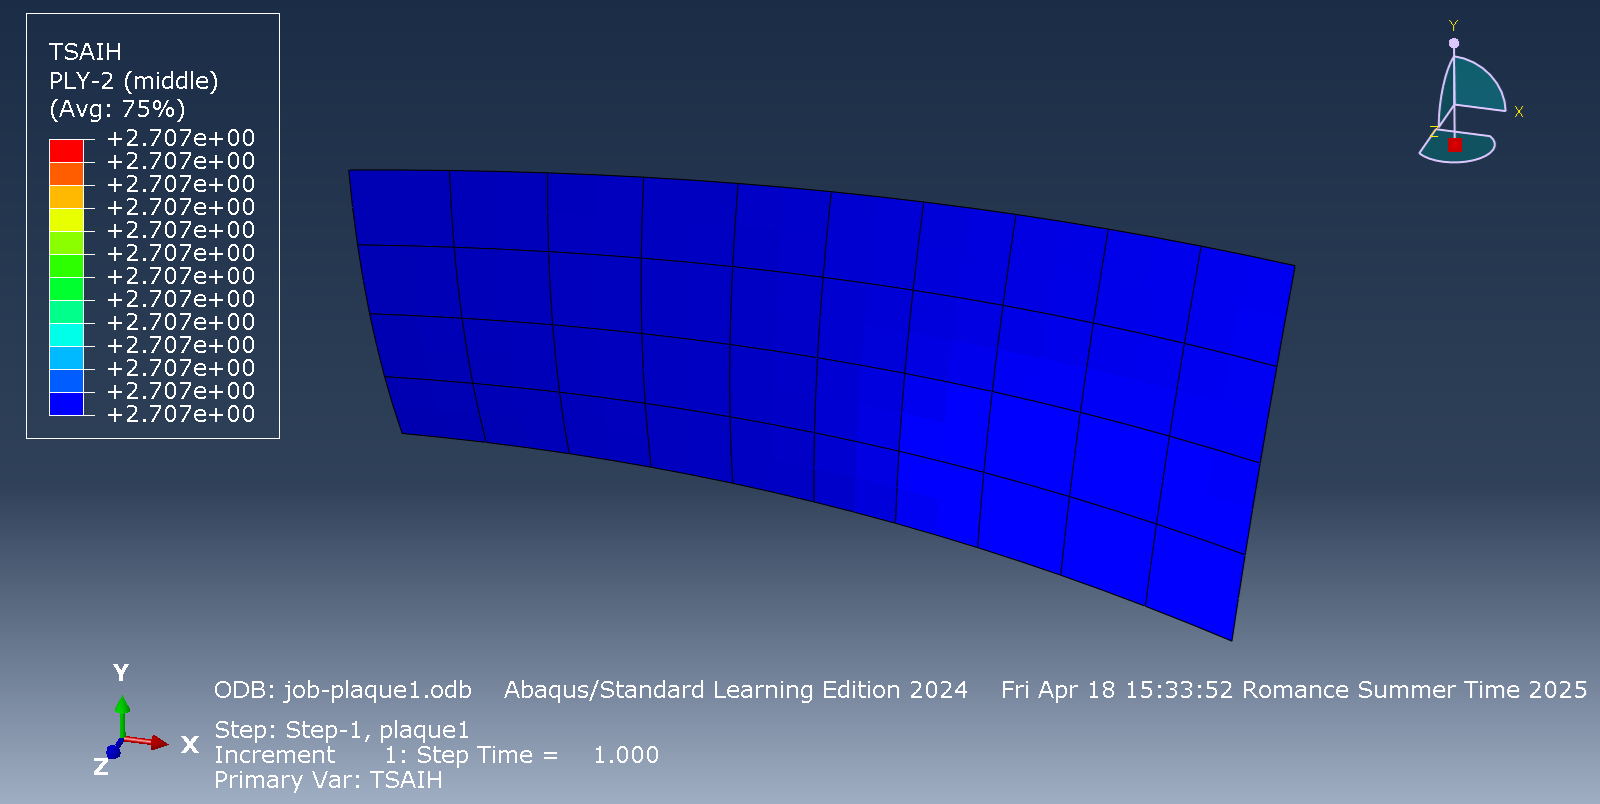
\includegraphics[width=\textwidth]{media/Couche2_.png} % Remplacez par le chemin de votre deuxième image
		\caption{Couche 2, plaque rectangle (William)}
		\label{fig:image2}
	\end{minipage}
\end{figure}
\clearpage

%résultats de la plaque 1, couche 3
\begin{figure}[h!]
	\centering
	\begin{minipage}{0.495\textwidth}
		\centering
		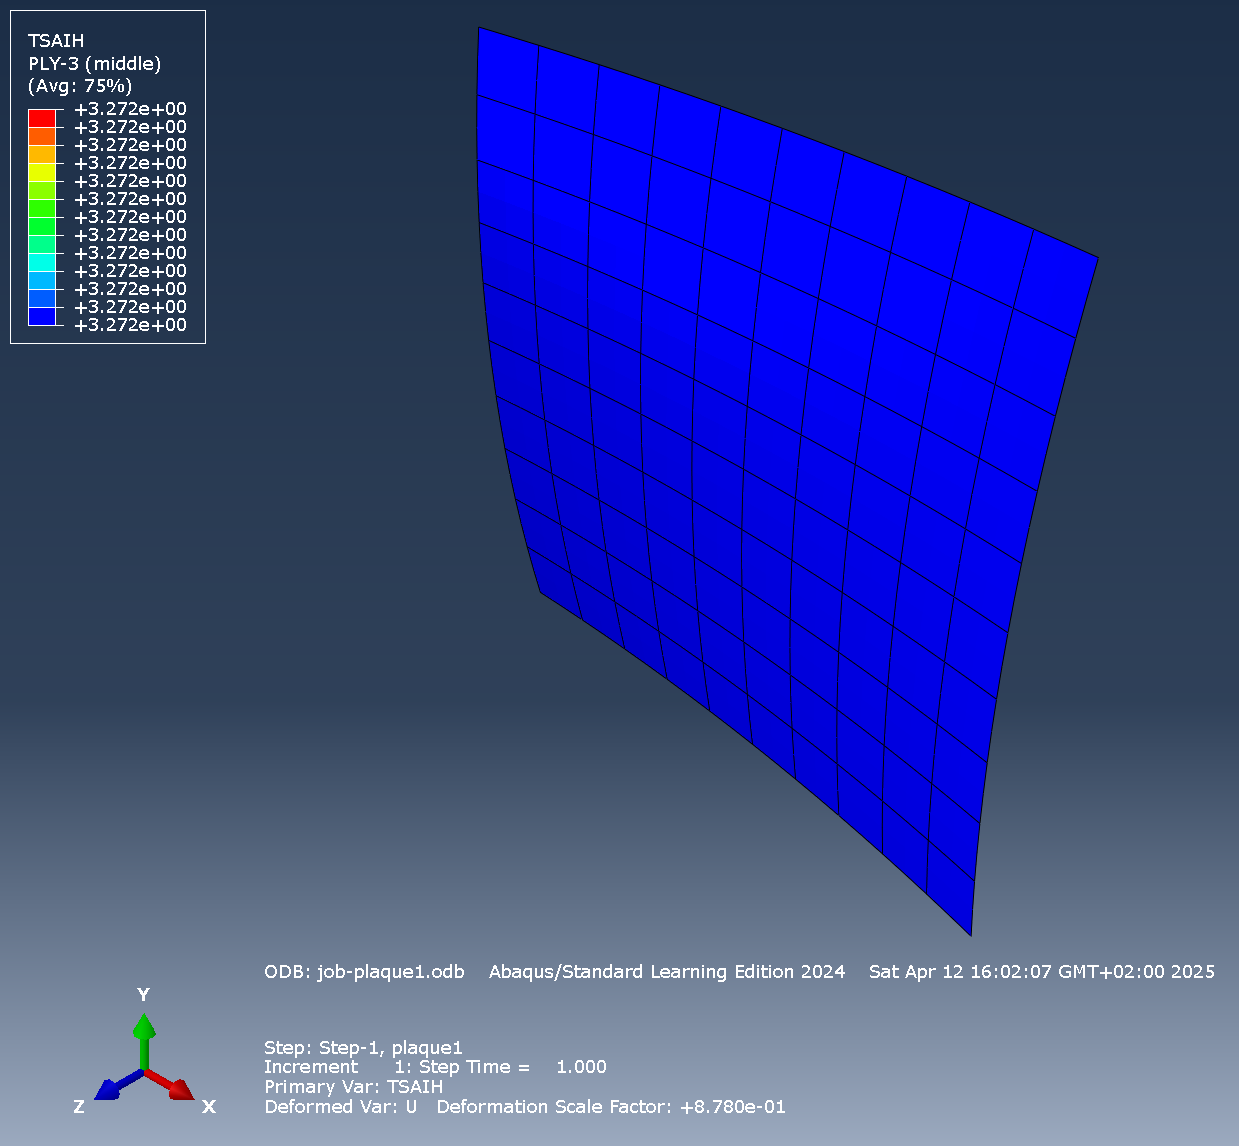
\includegraphics[width=\textwidth]{media/K_P1_L3_12042025.png} % Remplacez par le chemin de votre première image
		\caption{Couche 3, plaque carrée (Killian)}
		\label{fig:image1}
	\end{minipage}
	\hfill
	\begin{minipage}{0.495\textwidth}
		\centering
		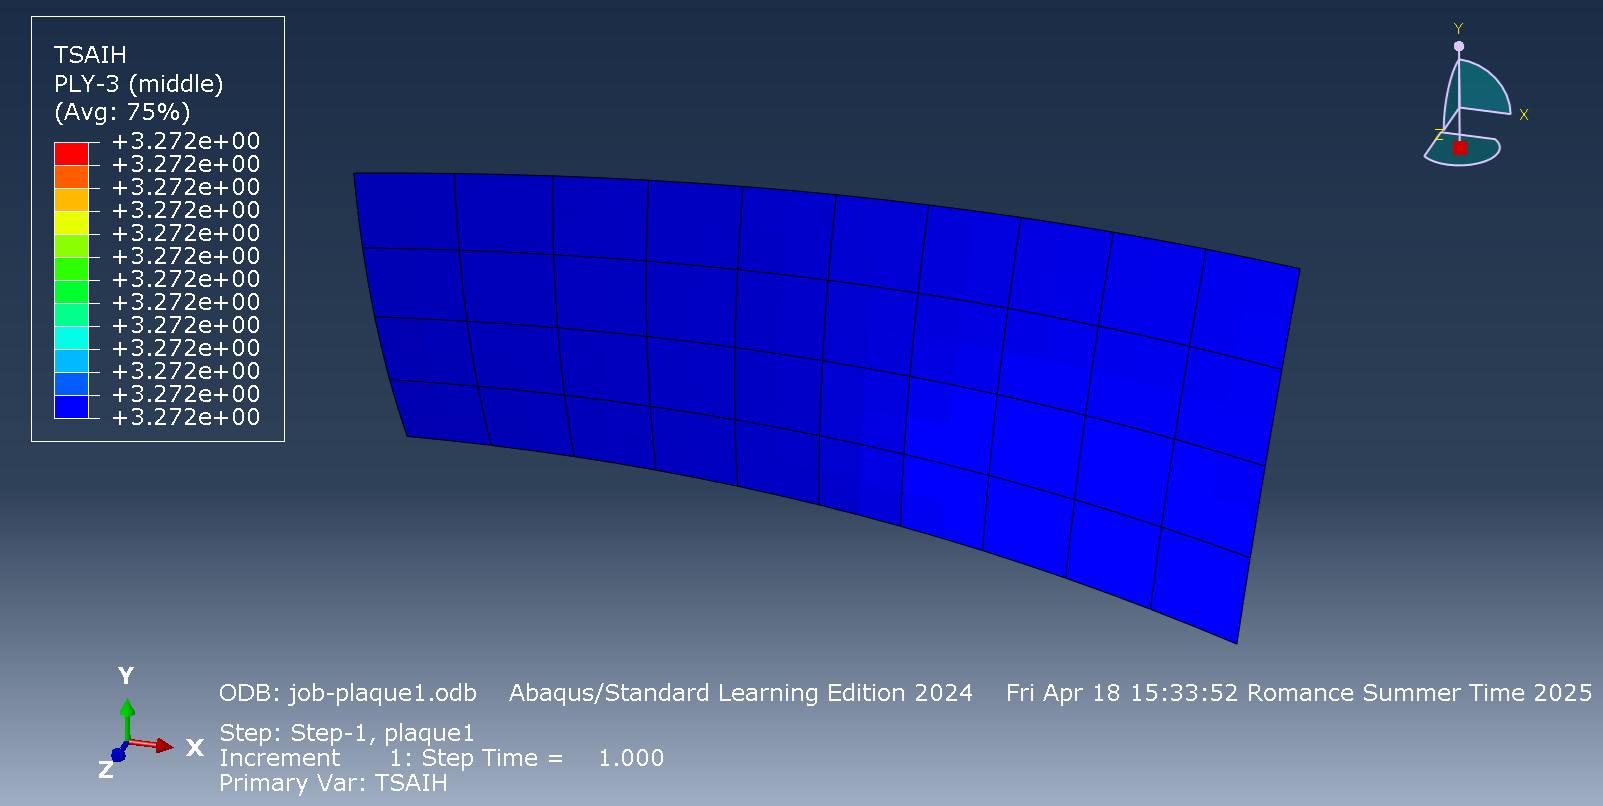
\includegraphics[width=\textwidth]{media/Couche3_.png} % Remplacez par le chemin de votre deuxième image
		\caption{Couche 3, plaque rectangle (William)}
		\label{fig:image2}
	\end{minipage}
\end{figure}

%résultats de la plaque 1, couche 4
\begin{figure}[h!]
	\centering
	\begin{minipage}{0.495\textwidth}
		\centering
		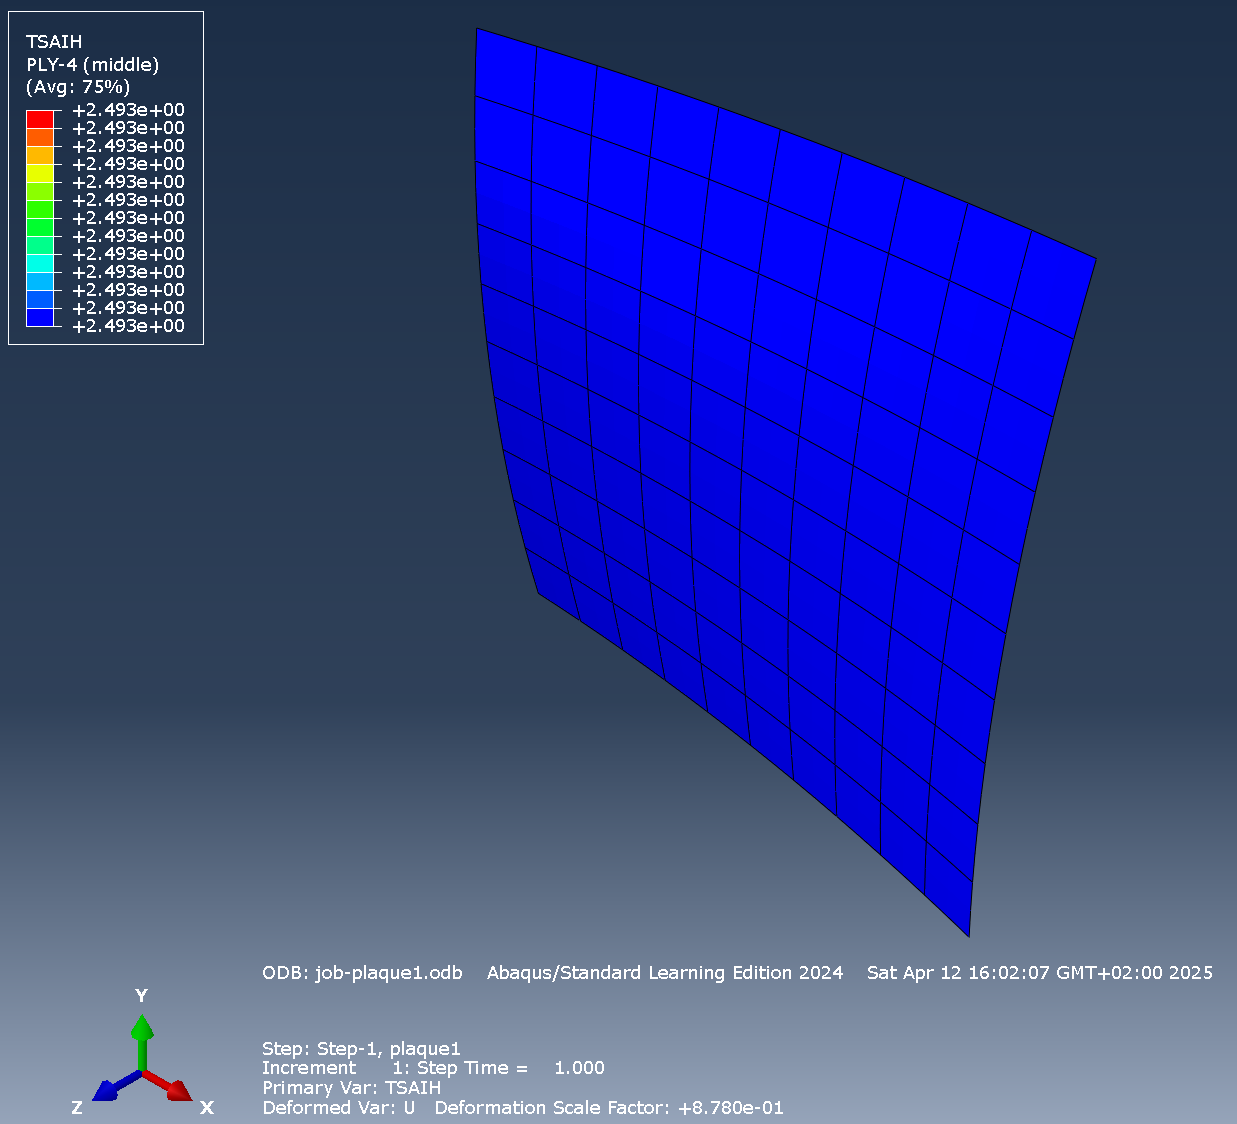
\includegraphics[width=\textwidth]{media/K_P1_L4_12042025.png} % Remplacez par le chemin de votre première image
		\caption{Couche 4, plaque carrée (Killian)}
		\label{fig:image1}
	\end{minipage}
	\hfill
	\begin{minipage}{0.495\textwidth}
		\centering
		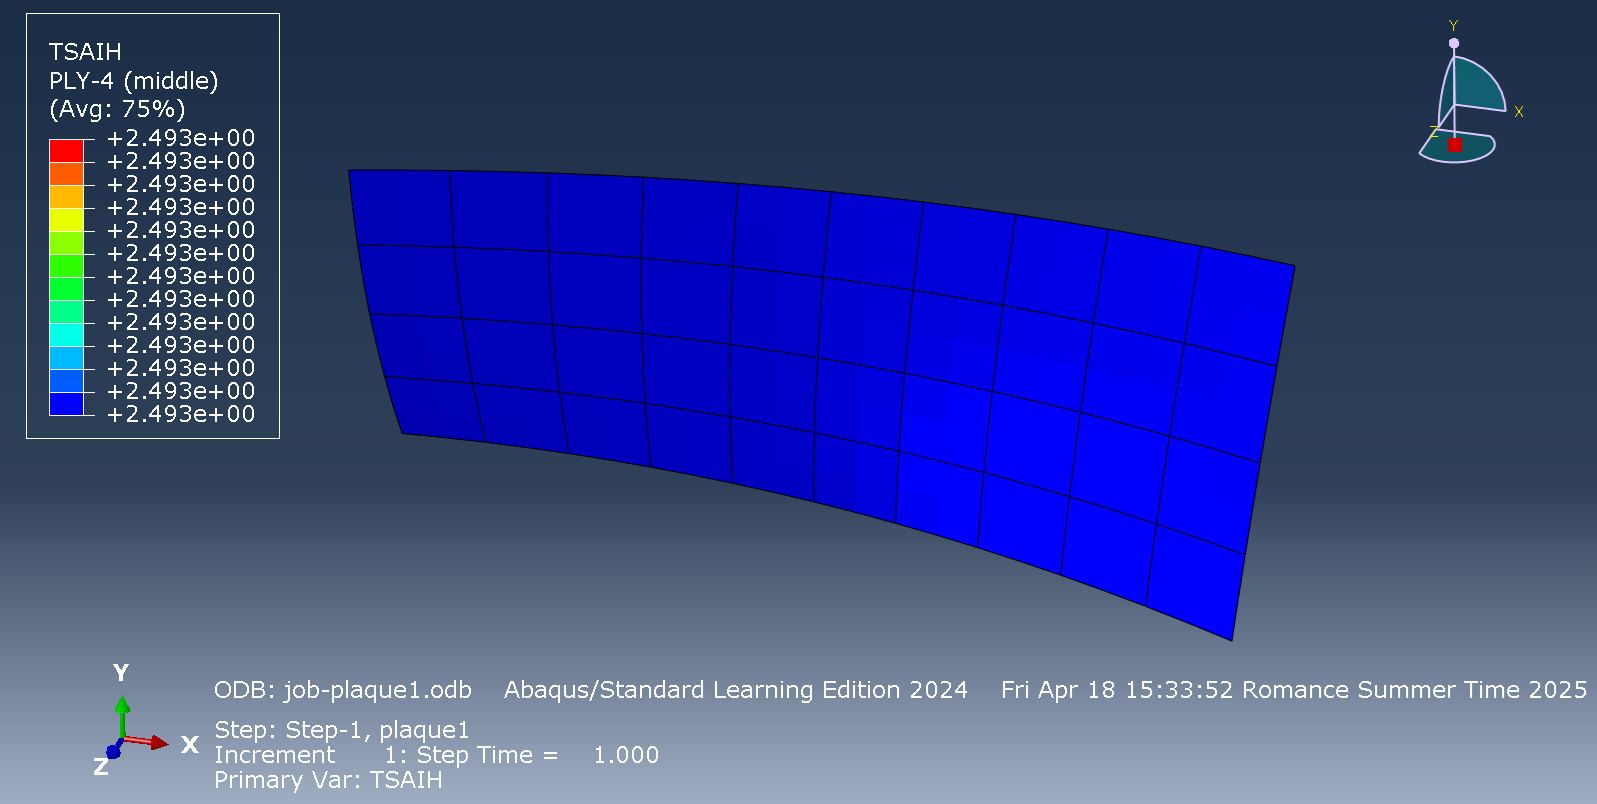
\includegraphics[width=\textwidth]{media/Couche4_.png} % Remplacez par le chemin de votre deuxième image
		\caption{Couche 4, plaque rectangle (William)}
		\label{fig:image2}
	\end{minipage}
\end{figure}



\subsection{Résultats obtenus avec la feuille de calcul composite}
Nous allons maintenant comparer les valeurs du critère de Tsai-Hill obtenues sous Abaqus avec celles obtenues avec la feuille de calcul composite conçue lors du premier TP de structures composites.

\begin{table}[h]
	\centering
	\begin{tabular}{|l|c|c|c|c|c|c|c|c|}
	\hline
	\textbf{Couche} & \multicolumn{2}{c|}{1} & \multicolumn{2}{c|}{2} & \multicolumn{2}{c|}{3} & \multicolumn{2}{c|}{4} \\ \hline
	\textbf{Orientation (°)} & \multicolumn{2}{c|}{30} & \multicolumn{2}{c|}{-15} & \multicolumn{2}{c|}{-30} & \multicolumn{2}{c|}{15} \\ \hline
	\textbf{z (mm)} & 2.5 & 1.5 & 1.5 & 0 & 0 & -1 & -1 & -2.5 \\ \hline
	\multicolumn{9}{|c|}{\textbf{Résultats Abaqus}} \\ \hline
	\textbf{Tsai-Hill (milieu)} & \multicolumn{2}{c|}{1.642} & \multicolumn{2}{c|}{2.707} & \multicolumn{2}{c|}{3.272} & \multicolumn{2}{c|}{2.493} \\ \hline
	\multicolumn{9}{|c|}{\textbf{Résultats feuille calcul TP1}} \\ \hline
	\textbf{Tsai-Hill (sup./inf.)} & 1.642 & 1.704 & 2.443 & 2.927 & 3.131 & 3.451 & 2.381 & 2.696 \\ \hline
	\end{tabular}
	\caption{Comparaison des résultats pour la plaque carrée (Killian)}
	\label{fig:Comparaison plaque carrée}
\end{table}

Il est impportant de remarquer que la feuille de calcul nous donne les valeurs du critère de Tsai-Hill pour les surfaces supérieures et inférieures de la plaque, alors qu'Abaqus nous donne les valeurs pour le milieu de la couche. Cependant les résultats sont cohérents car la valeur du critère de rupture en milieu de couche est toujours comprise entre les valeurs de la surface supérieure et inférieure. 

\subsection{Conclusion vis-à-vis du dimensionnement de la plaque 1}
Nous constatons que le critère de Tsai-Hill est dépassé (>1) pour toutes les couches de la plaque 1, ce qui signifie que la plaque 1 ne peut pas être utilisée dans ces conditions de chargement. Il est donc nécessaire de modifier l'orientation des couches ou d'augmenter l'épaisseur de la plaque pour respecter le critère de rupture.

\subsection {Optimisation de la plaque pour répondre au cahier des charges.}
Si nous voulons atteindre le critère de rupture inférieur à 1 pour toutes les couches nous avons dans un premier temps éssayé de faire varier l'épaisseur de celles-ci. Nous avons donc pris la plaque 1 et nous avons modifié l'épaisseur de chaque couche dans la feuille de calcul pour obtenir le tableau suivant:

\begin{table}[h!]
	\renewcommand{\arraystretch}{1.2} % Augmente l'interligne des lignes du tableau
	\centering
	\begin{tabular}{c|c|c}
		\textbf{N° pli} & \textbf{Orientation (°)} & \textbf{Epaisseur (mm)} \\
		\hline
		4         & 15              & 6.5           \\
		3          & -30              & 1.5           \\
		2          & -15              & 1          \\
		1         & 30             & 4.5         \\
	\end{tabular}
	\caption{Lay-up de la plaque 1 asymétrique supportant le chargement}
	\label{tab:lay up opti epaisseur}
\end{table}

Il est donc nécessaire d'avoir une plaque d'épaisseur 13.5 mm pour que celle-ci résiste au chargement sans changer l'orientation des couches. C'est à dire qu'il faut presque doubler son épaisseur, ce qui peut être un lourd inconvénient en terme d'espace utilisé. Nous allons donc essayer d'obtenir une épaisseur plus faible en changeant l'orientation des couches. 



\begin{table}[H]
	\renewcommand{\arraystretch}{1.2} % Augmente l'interligne des lignes du tableau
	\centering
	\begin{tabular}{c|c|c}
		\textbf{N° pli} & \textbf{Orientation (°)} & \textbf{Epaisseur (mm)} \\
		\hline
		4         & -10              & 2           \\
		3          & 55              & 1           \\
		2          & 55            & 3          \\
		1         & -10             & 2        \\
	\end{tabular}
	\caption{Lay-up optimisé de la plaque 1 asymétrique supportant le chargement}
	\label{tab:lay up opti epaisseur orientation}
\end{table}

Cette combinaison de paramètres nous permet donc d'obtenir environ 8 mm d'épaisseur total, soit 5,5 mm de moins que la plaque où nous avons seulement modifié l'épaisseur.
On peut donc clairement conclure sur le fait que l'orientation des couches joue un role majeur dans la solidité des plaques.
%Plaque 2

\section{Plaque 4 plis avec symétrie miroir sous chargement mécanique}
\subsection{Hypothèses nécessaires à la mise en place du modèle numérique}
Les hypothèses nécessaires à la mise en place du modèle numérique de la plaque 2 sont les mêmes que pour la plaque 1, à l'exception que la plaque 2 est symétrique par rapport au plan médian.
(Table \ref{Tableau 1: Hypothèses pour la plaque 1})

\subsection{Mise en place du modèle numérique sous Abaqus}
Les hypothèses nous ont permis de mettre en place le modèle numérique de la plaque 2 en considérant l'empilement suivant:

\begin{table}[h!]
	\renewcommand{\arraystretch}{1.2} % Augmente l'interligne des lignes du tableau
	\centering
	\begin{tabular}{c|c|c}
		\textbf{N° pli} & \textbf{Orientation (°)} & \textbf{Epaisseur (mm)} \\
		\hline
		1'         & 30             & 1           \\
		2'          & -15              & 1,5           \\
		3'          & -30              & 1            \\
		4'         & 15              & 1,5            \\
		\hline
		Symétrie miroir \\
		\hline
		4         & 15              & 1,5            \\
		3          & -30              & 1            \\
		2          & -15              & 1,5           \\
		1         & 30             & 1           \\
	\end{tabular}
	\caption{Lay-up de la plaque 1 asymétrique}
	\label{tab:exemple_tableau}
\end{table}

\begin{figure}[h!]
	\centering
	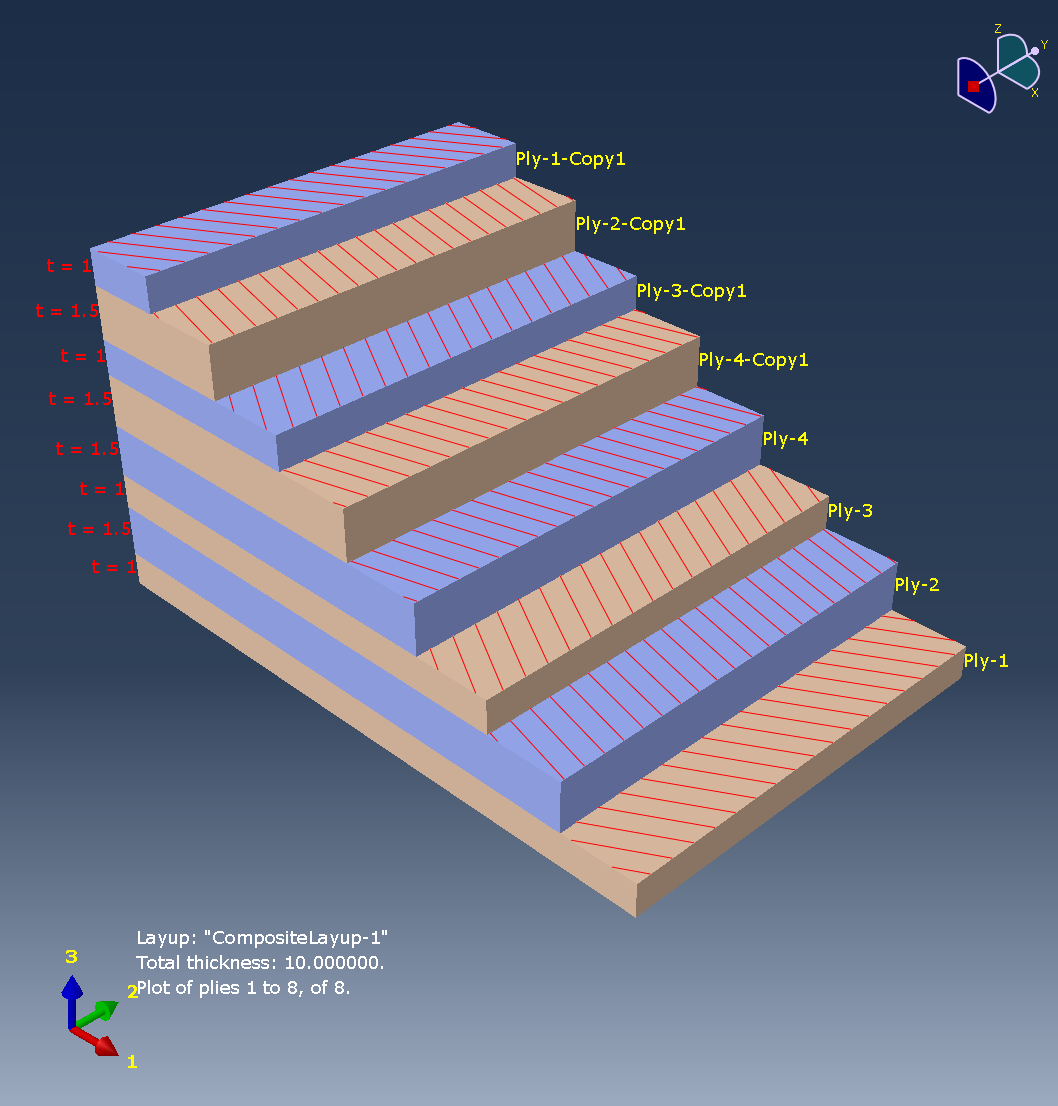
\includegraphics[width=0.5\textwidth]{media/K_P2_layout_12042025.png} % Remplacez par le chemin de votre image
	\caption{Lay-up de la plaque 2 visualisé sous Abaqus.}
	\label{fig:exemple_image}
\end{figure}

\subsection{Résultats obtenus sous Abaqus}

La plaque étant symétrique nous allons simplement afficher les résultats des couches 1 à 4, les valeurs du critère de Tsai-Hill étant identiques pour les couches conjuguées (4=4', 3=3', 2=2', 1=1').

%résultats de la plaque 2, couche 1
\begin{figure}[H]
	\centering
	\begin{minipage}[t][0.3\textheight]{0.495\textwidth}
		\centering
		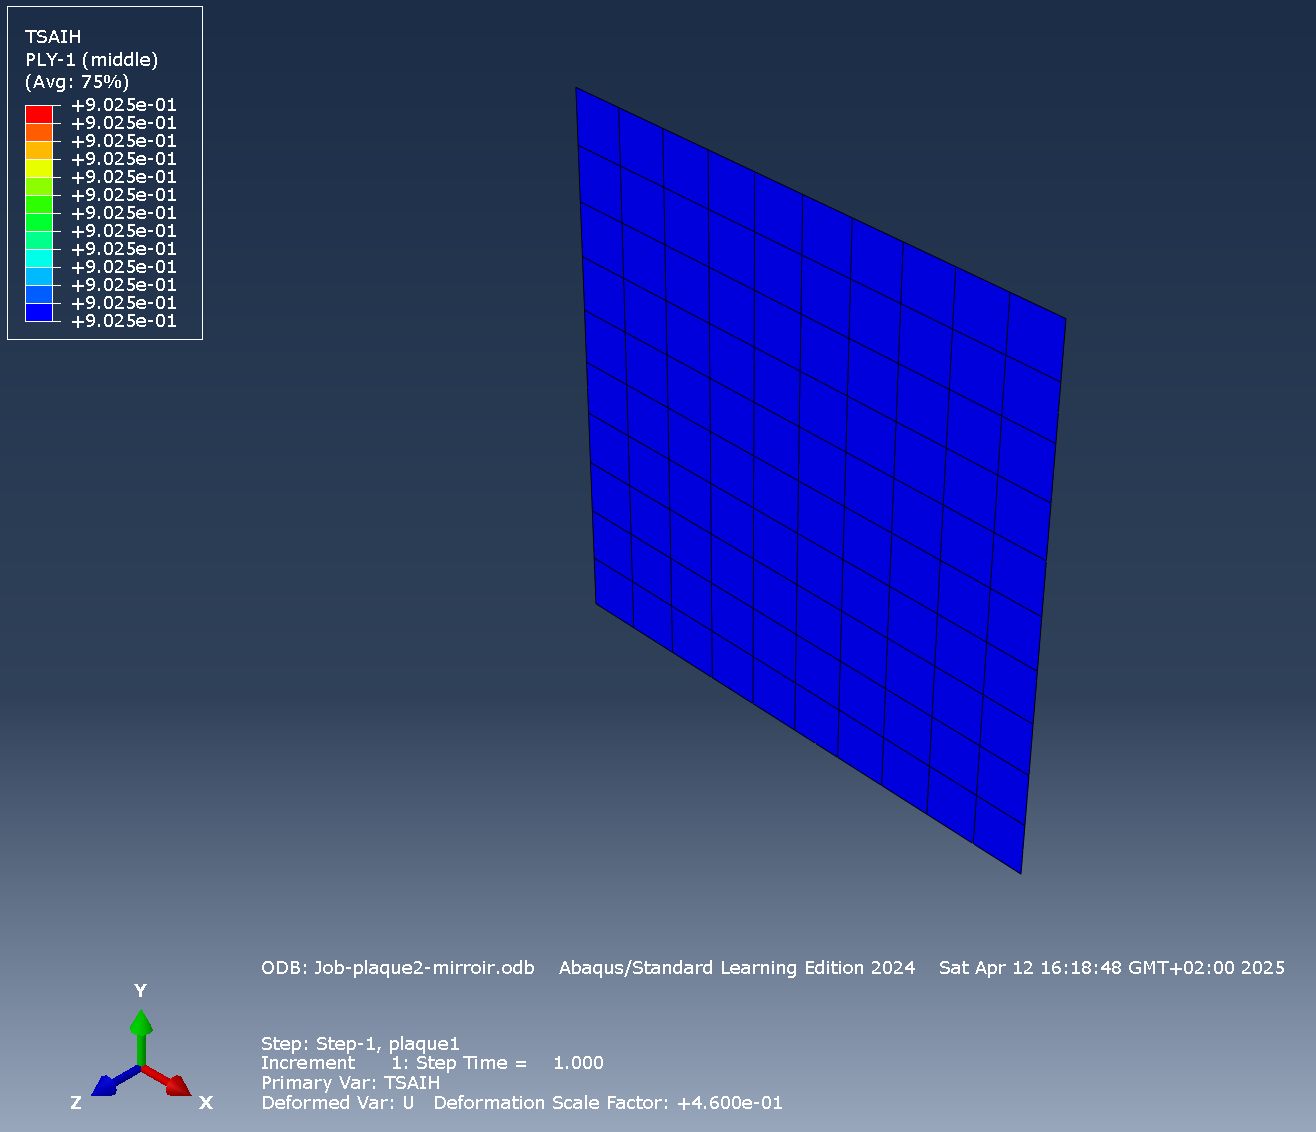
\includegraphics[width=\textwidth]{media/K_P2_L1-8_12042025.png} % Remplacez par le chemin de votre première image
		\caption{Couche 1, plaque carrée (Killian)}
		\label{fig:image1}
	\end{minipage}
	\hfill
	\begin{minipage}[t][0.3\textheight]{0.495\textwidth}
		\centering
		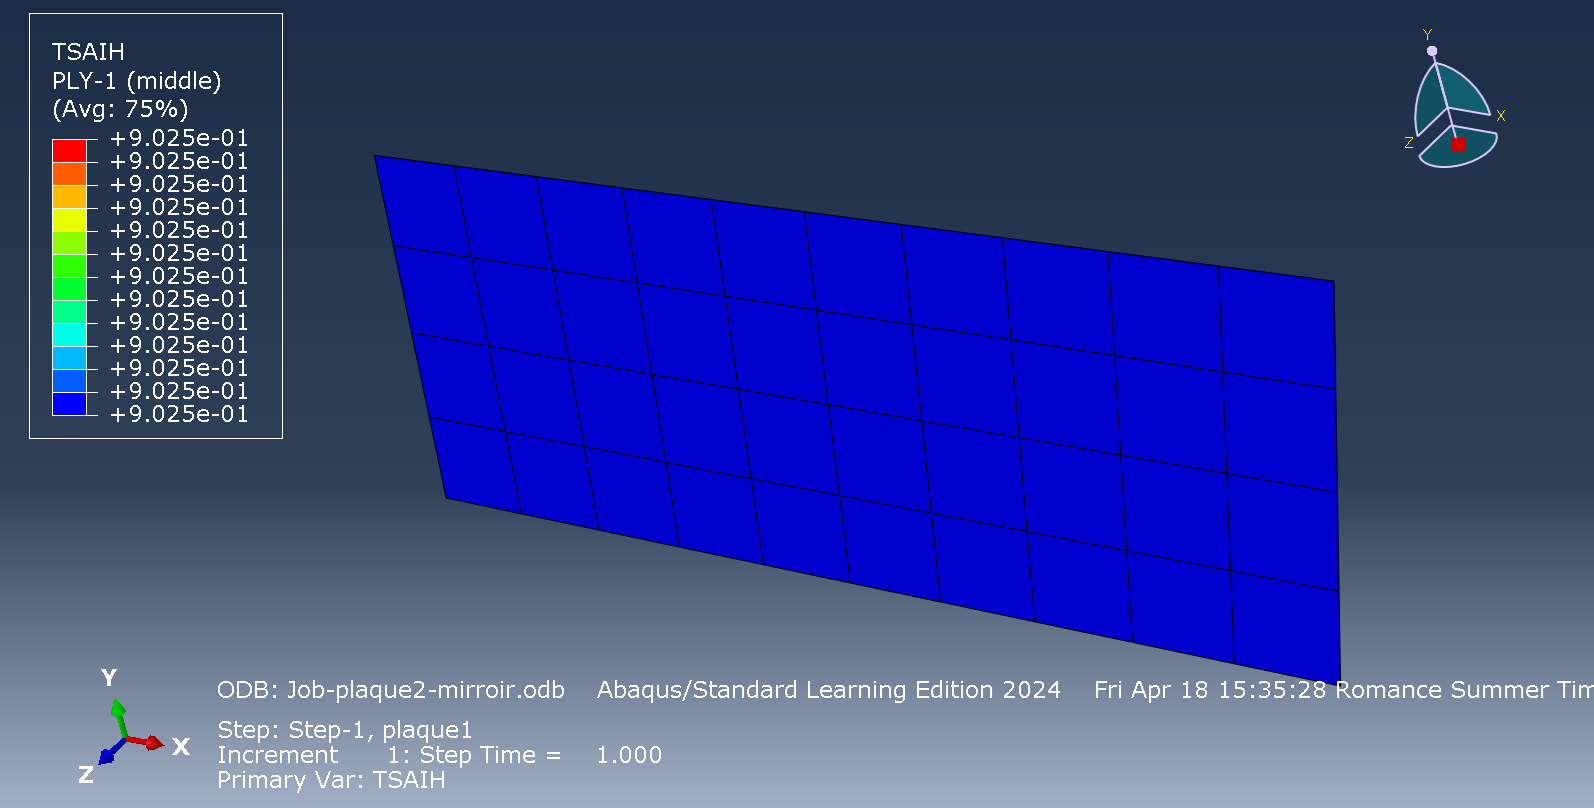
\includegraphics[width=\textwidth]{media/Couche1_Mirroir.png} % Remplacez par le chemin de votre deuxième image
		\caption{Couche 1, plaque rectangle (William)}
		\label{fig:image2}
	\end{minipage}
\end{figure}

%résultats de la plaque 2, couche 2
\begin{figure}[H]
	\centering
	\begin{minipage}[t][0.3\textheight]{0.495\textwidth}
		\centering
		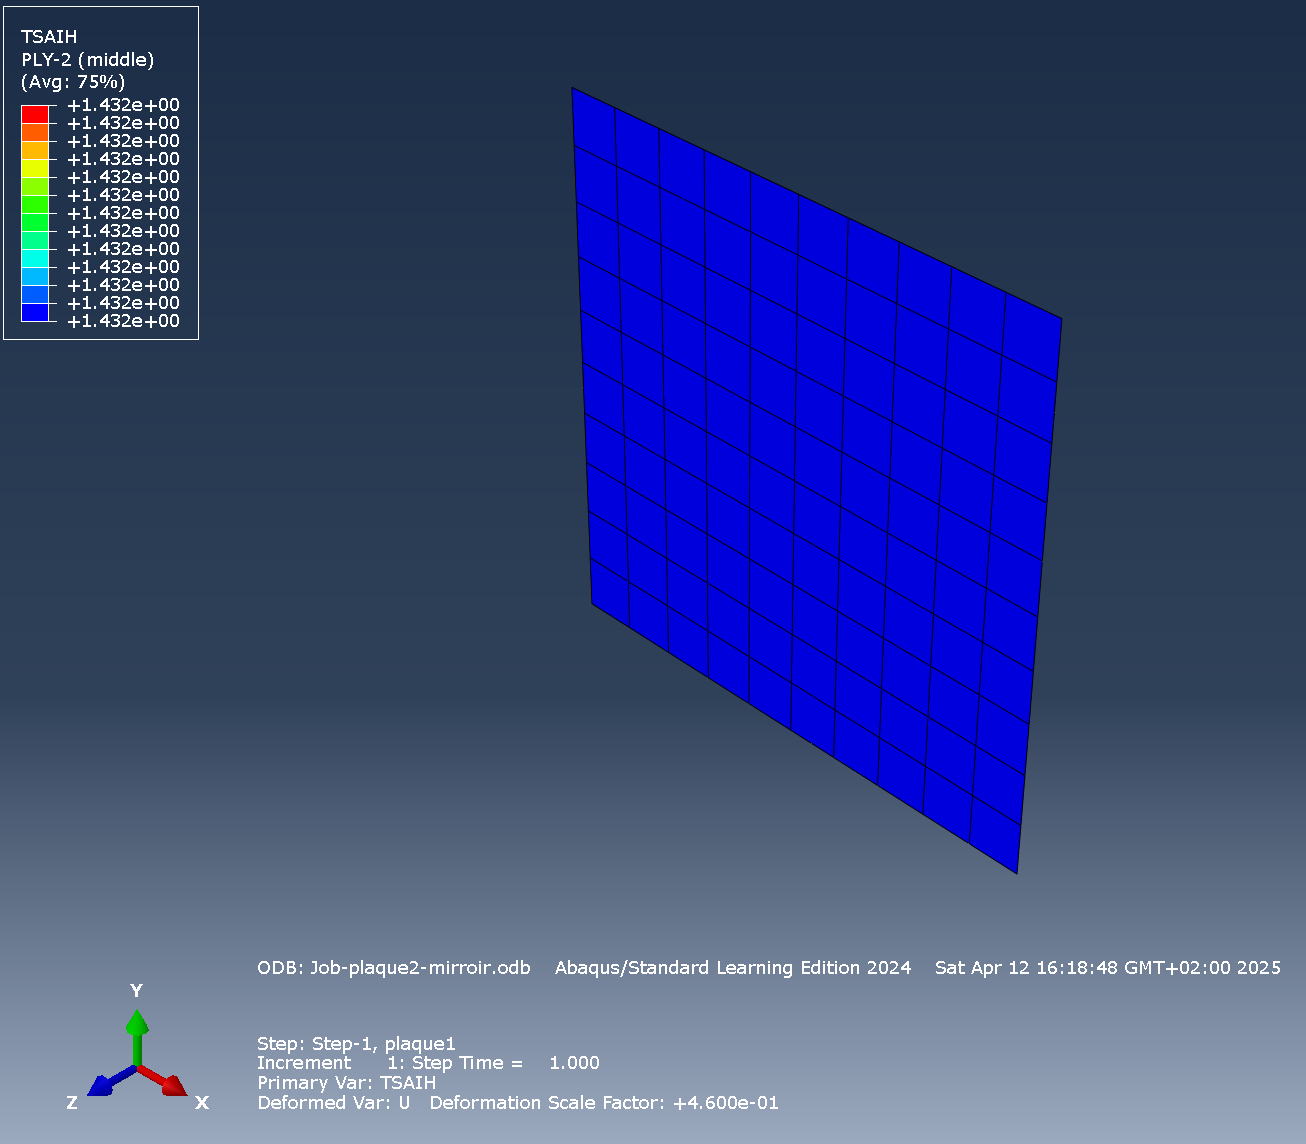
\includegraphics[width=\textwidth]{media/K_P2_L2-7_12042025.png} % Remplacez par le chemin de votre première image
		\caption{Couche 2, plaque carrée (Killian)}
		\label{fig:image1}
	\end{minipage}
	\hfill
	\begin{minipage}[t][0.3\textheight]{0.495\textwidth}
		\centering
		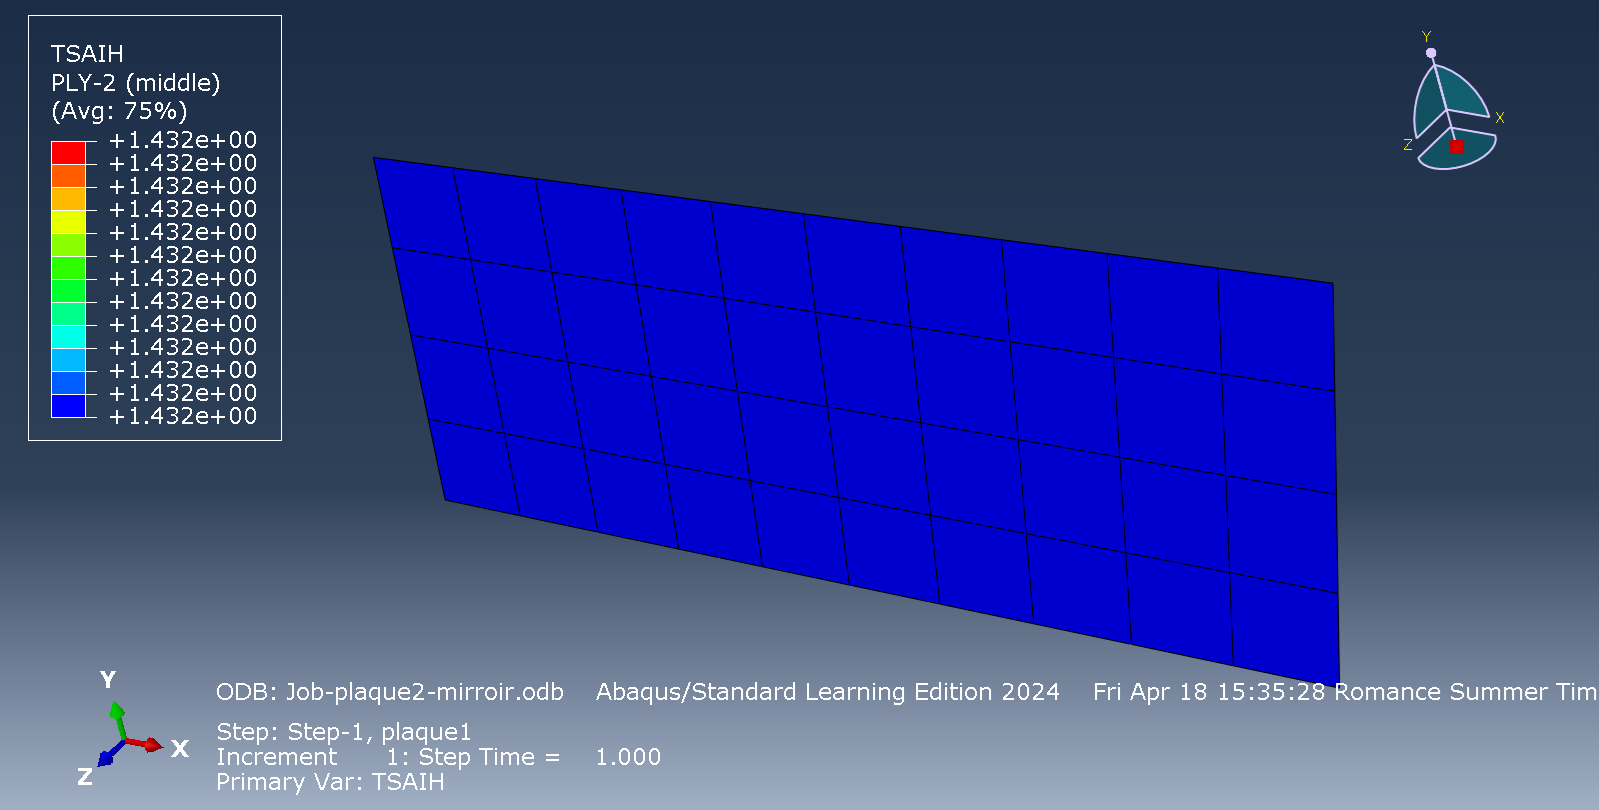
\includegraphics[width=\textwidth]{media/Couche2_mirroir.png} % Remplacez par le chemin de votre deuxième image
		\caption{Couche 2, plaque rectangle (William)}
		\label{fig:image2}
	\end{minipage}
\end{figure}


%résultats de la plaque 2, couche 3
\begin{figure}[H]
	\centering
	\begin{minipage}{0.495\textwidth}
		\centering
		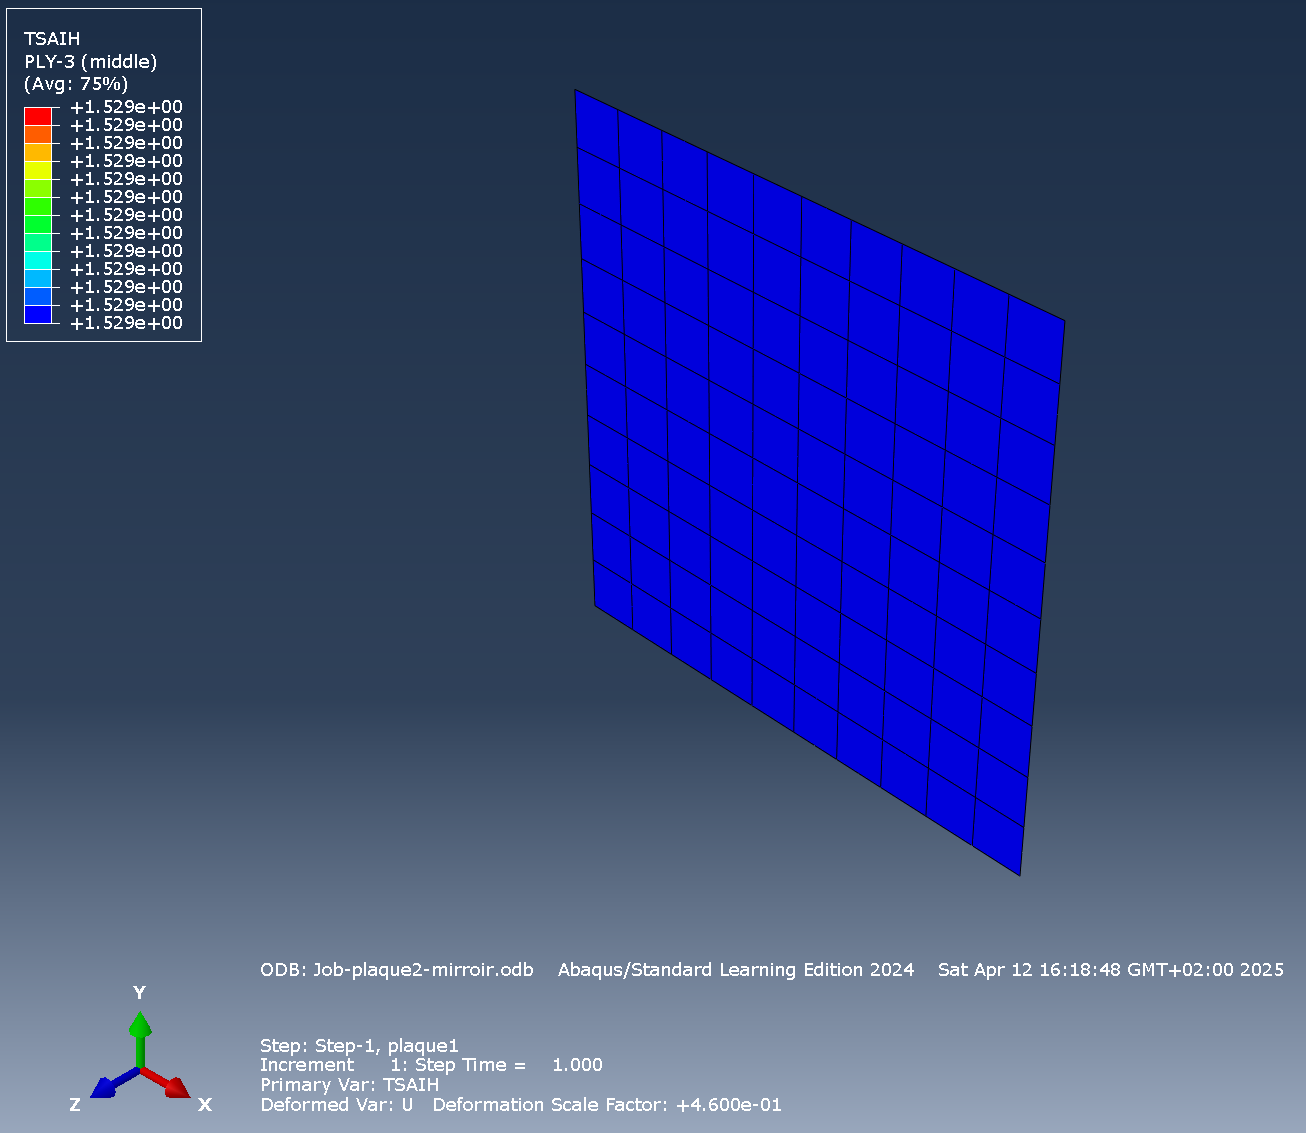
\includegraphics[width=\textwidth]{media/K_P2_L3-6_12042025.png} % Remplacez par le chemin de votre première image
		\caption{Couche 3, plaque carrée (Killian)}
		\label{fig:image1}
	\end{minipage}
	\hfill
	\begin{minipage}{0.495\textwidth}
		\centering
		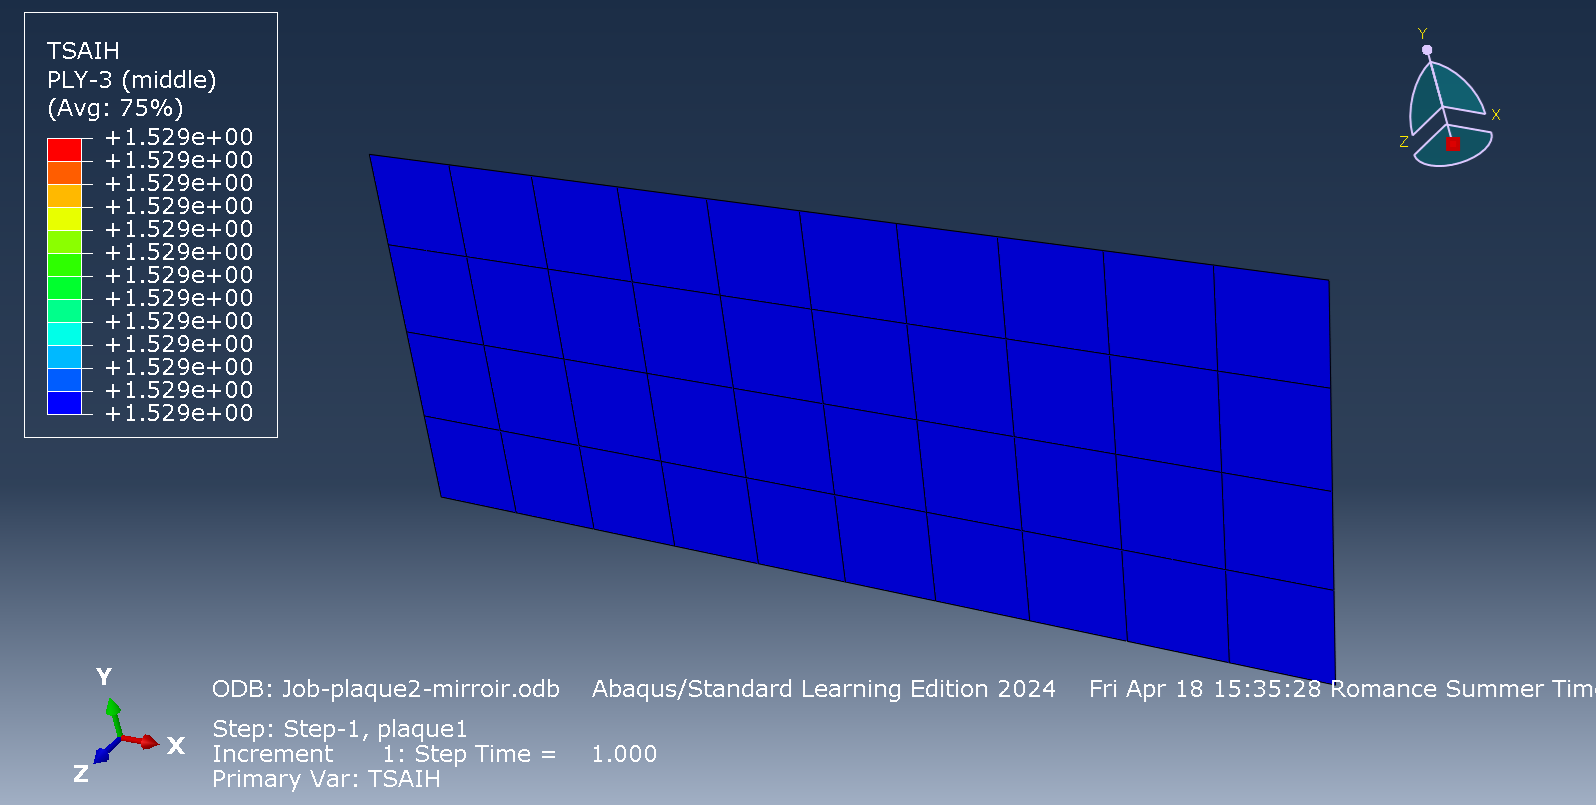
\includegraphics[width=\textwidth]{media/Couche3_mirroir.png} % Remplacez par le chemin de votre deuxième image
		\caption{Couche 3, plaque rectangle (William)}
		\label{fig:image2}
	\end{minipage}
\end{figure}

%résultats de la plaque 2, couche 4
\begin{figure}[H]
	\centering
	\begin{minipage}{0.495\textwidth}
		\centering
		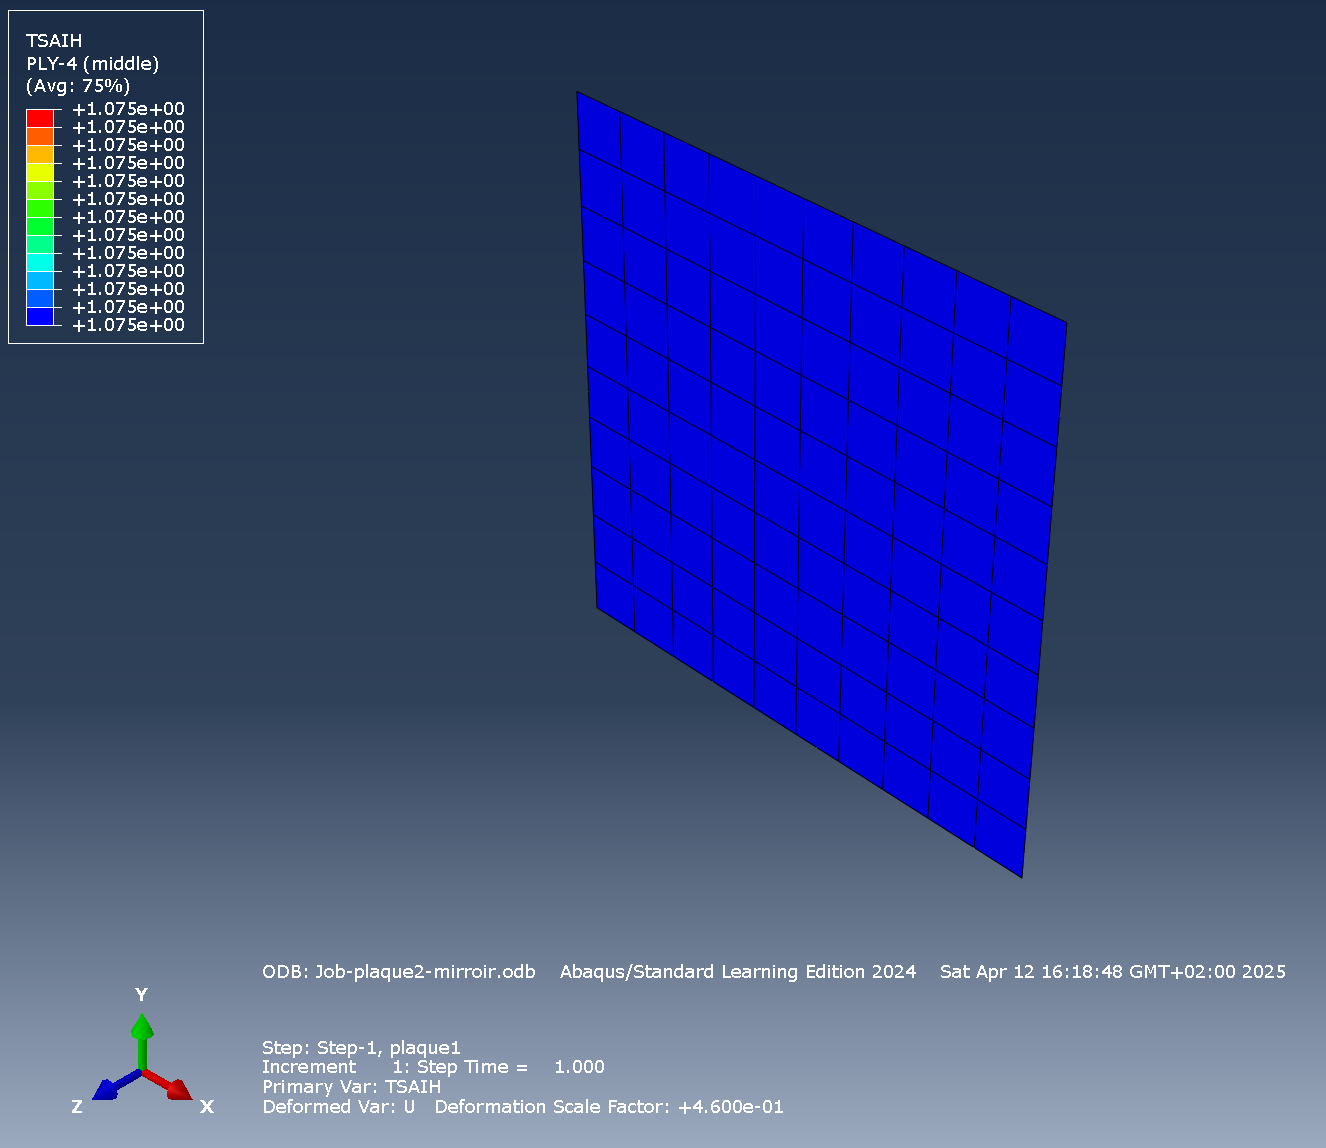
\includegraphics[width=\textwidth]{media/K_P2_L4-5_12042025.png} % Remplacez par le chemin de votre première image
		\caption{Couche 4, plaque carrée (Killian)}
		\label{fig:image1}
	\end{minipage}
	\hfill
	\begin{minipage}{0.495\textwidth}
		\centering
		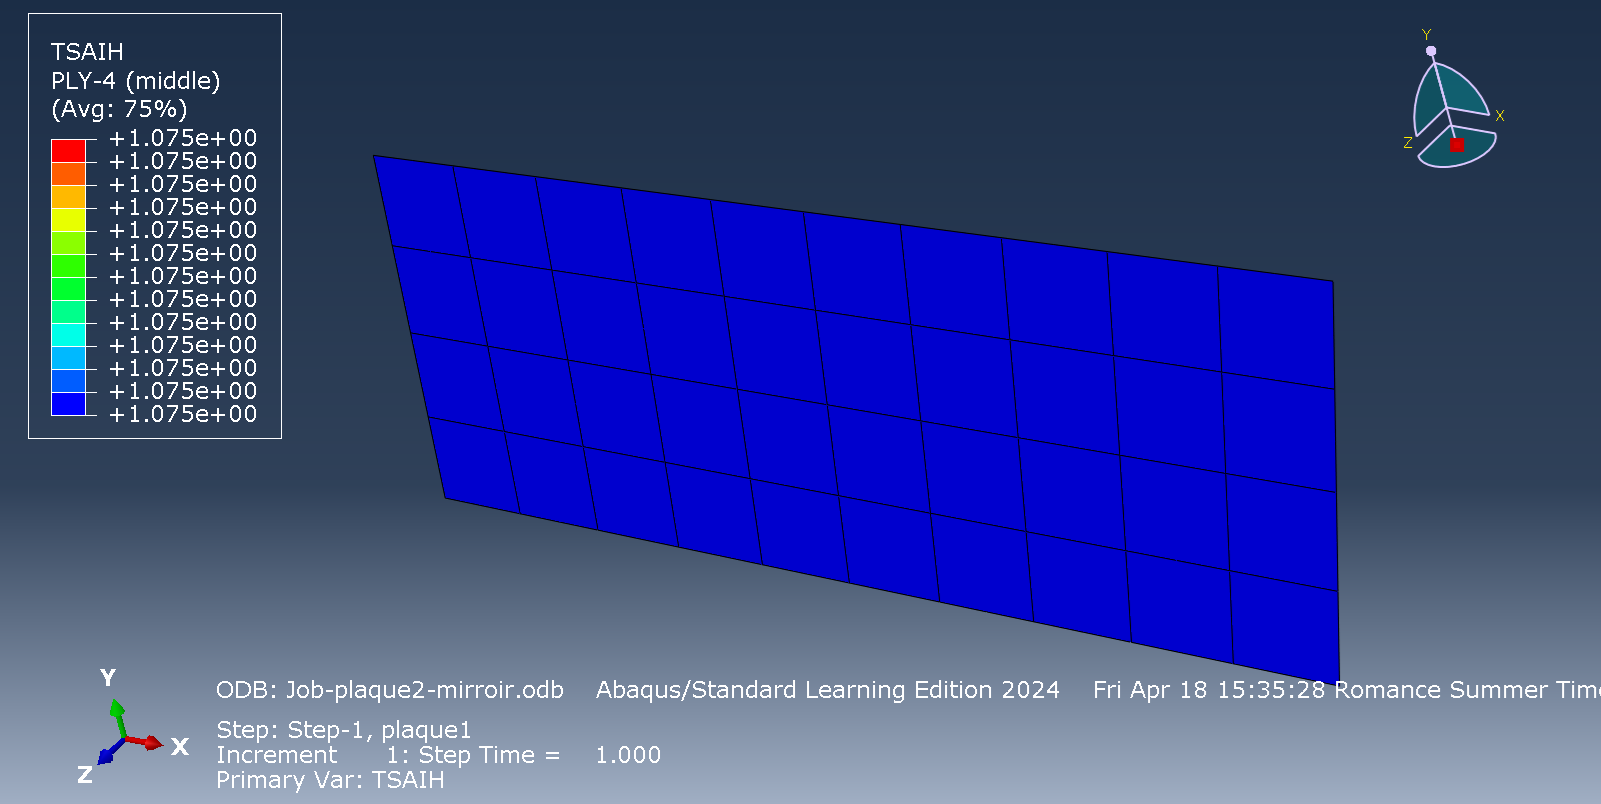
\includegraphics[width=\textwidth]{media/Couche4_mirroir.png} % Remplacez par le chemin de votre deuxième image
		\caption{Couche 4, plaque rectangle (William)}
		\label{fig:image2}
	\end{minipage}
\end{figure}



\subsection{Résultats obtenus avec la feuille de calcul composite}
Nous allons maintenant comparer les valeurs du critère de Tsai-Hill obtenues sous Abaqus avec celles obtenues avec la feuille de calcul composite conçue lors du premier TP de structures composites.

\begin{table}[h]
	\centering
	\begin{tabular}{|l|c|c|c|c|c|c|c|c|}
	\hline
	\textbf{Couche} & \multicolumn{2}{c|}{1 - 1'} & \multicolumn{2}{c|}{2 - 2'} & \multicolumn{2}{c|}{3 - 3'} & \multicolumn{2}{c|}{4 - 4'} \\ \hline
	\textbf{Orientation (°)} & \multicolumn{2}{c|}{30} & \multicolumn{2}{c|}{-15} & \multicolumn{2}{c|}{-30} & \multicolumn{2}{c|}{15} \\ \hline
	\textbf{z (mm)} & 2.5 & 1.5 & 1.5 & 0 & 0 & -1 & -1 & -2.5 \\ \hline
	\multicolumn{9}{|c|}{\textbf{Résultats Abaqus}} \\ \hline
	\textbf{Tsai-Hill (milieu)} & \multicolumn{2}{c|}{0.902} & \multicolumn{2}{c|}{1.432} & \multicolumn{2}{c|}{1.529} & \multicolumn{2}{c|}{1.07} \\ \hline
	\multicolumn{9}{|c|}{\textbf{Résultats feuille calcul TP1}} \\ \hline
	\textbf{Tsai-Hill (sup./inf.)} & 0.902 & 0.902 & 1.432 & 1.432 & 1.529 & 1.529 &  1.075 &  1.075 \\ \hline
	\end{tabular}
	\caption{Comparaison des résultats pour la plaque carrée }
	\label{fig:Comparaison plaque carrée}
\end{table}

\subsection{Conclusion vis-à-vis du dimensionnement de la plaque 2}
Nous constatons que le critère de Tsai-Hill est dépassé (>1) pour certaines couches de la plaque , ce qui signifie que la plaque 2 ne peut pas être utilisée dans ces conditions de chargement. Il est donc nécessaire de modifier l'orientation des couches ou d'augmenter l'épaisseur de la plaque pour respecter le critère de rupture.

\subsection {Optimisation de la plaque pour répondre au cahier des charges}
Si nous voulons atteindre le crtitère de rupture inférieur à 1 pour toutes les couches nous avons dans un premier temps essayé de faire varier l'épaisseur de celles-ci. Nous avons donc pris la plaque 2 et nous avons modifié l'épaisseur de chaque couche dans la feuille de calcul pour obtenir le tableau suivant:

\begin{table}[h!]
	\renewcommand{\arraystretch}{1.2} % Augmente l'interligne des lignes du tableau
	\centering
	\begin{tabular}{c|c|c}
		\textbf{N° pli} & \textbf{Orientation (°)} & \textbf{Epaisseur (mm)} \\
		\hline
		1'         & 30             & 2.5         \\
		2'          & -15              & 1          \\
		3'          & -30              & 1            \\
		4'         & 15              & 2            \\
		4         & 15              & 2            \\
		3          & -30              & 1            \\
		2          & -15              & 1          \\
		1         & 30             & 2.5         \\
	\end{tabular}
	\caption{Lay-up de la plaque 2 symétrique supportant le chargement}
	\label{tab:lay up opti epaisseur}
\end{table}

Il est donc nécessaire d'avoir une plaque d'épaisseur 13 mm pour que celle-ci résiste au chargement sans changer l'orientation des couches.

\begin{table}[h!]
	\renewcommand{\arraystretch}{1.2} % Augmente l'interligne des lignes du tableau
	\centering
	\begin{tabular}{c|c|c}
		\textbf{N° pli} & \textbf{Orientation (°)} & \textbf{Epaisseur (mm)} \\
		\hline
		1'         & 55             & 1        \\
		2'          & 55            & 1          \\
		3'          & -10             & 1           \\
		4'         & -10              & 1           \\
		4         & -10              & 1           \\
		3          & -10             & 1           \\
		2          & 55            & 1          \\
		1         & 55             & 1        \\
	\end{tabular}
	\caption{Lay-up optimisé de la plaque 2 symétrique supportant le chargement}
	\label{tab:lay up opti epaisseur orientation}
\end{table}

Cette variante des paramètres nous permet d'obtenir environ 8mm d'épaisseur, soit 5mm de moins que la dernière. Encore une fois, cela démontre bien l'importance de l'orientation des fibres dans chaque couches. De plus, on n'augmente que de 3mm l'epaisseur de la plaque originale pour qu'elle supporte le chargement.

%Plaque 3

\section{Plaque en acier sous chargement mécanique}
\subsection{Hypothèses nécessaires à la mise en place du modèle numérique}
Les hypothèses nécessaires à la mise en place du modèle numérique de la plaque 3 sont les mêmes que pour la plaque 1 (Table \ref{Tableau 1: Hypothèses pour la plaque 1}), à l'exception des éléments suivants:

\begin{table}[h!]
	\centering
	\renewcommand{\arraystretch}{1.2} % Augmente l'interligne des lignes du tableau
	\begin{tabular}{r p{10cm}}
		Matériau   & Acier Loi de comportement: linéaire élastique isotrope (E = 210 Gpa, $\nu$ = 0,28)\\
		\hline

		Section   & Coque Homogène, épaisseur 5 mm\\
		\hline
		Donnée de sortie   & U, $\sigma$, $\varepsilon$, Critère de rupture (Von Mises) \\
	\end{tabular}
	\caption{Hypothèses pour la plaque 3}
	\label{Tableau 1: Hypothèses pour la plaque 3}
\end{table}

\subsection{Mise en place du modèle numérique sous Abaqus}
Les hypothèses nous ont permis de mettre en place le modèle numérique de la plaque 3.

\subsection{Résultats obtenus sous Abaqus}



%résultats de la plaque 3
\begin{figure}[H]
	\centering
	\begin{minipage}{0.495\textwidth}
		\centering
		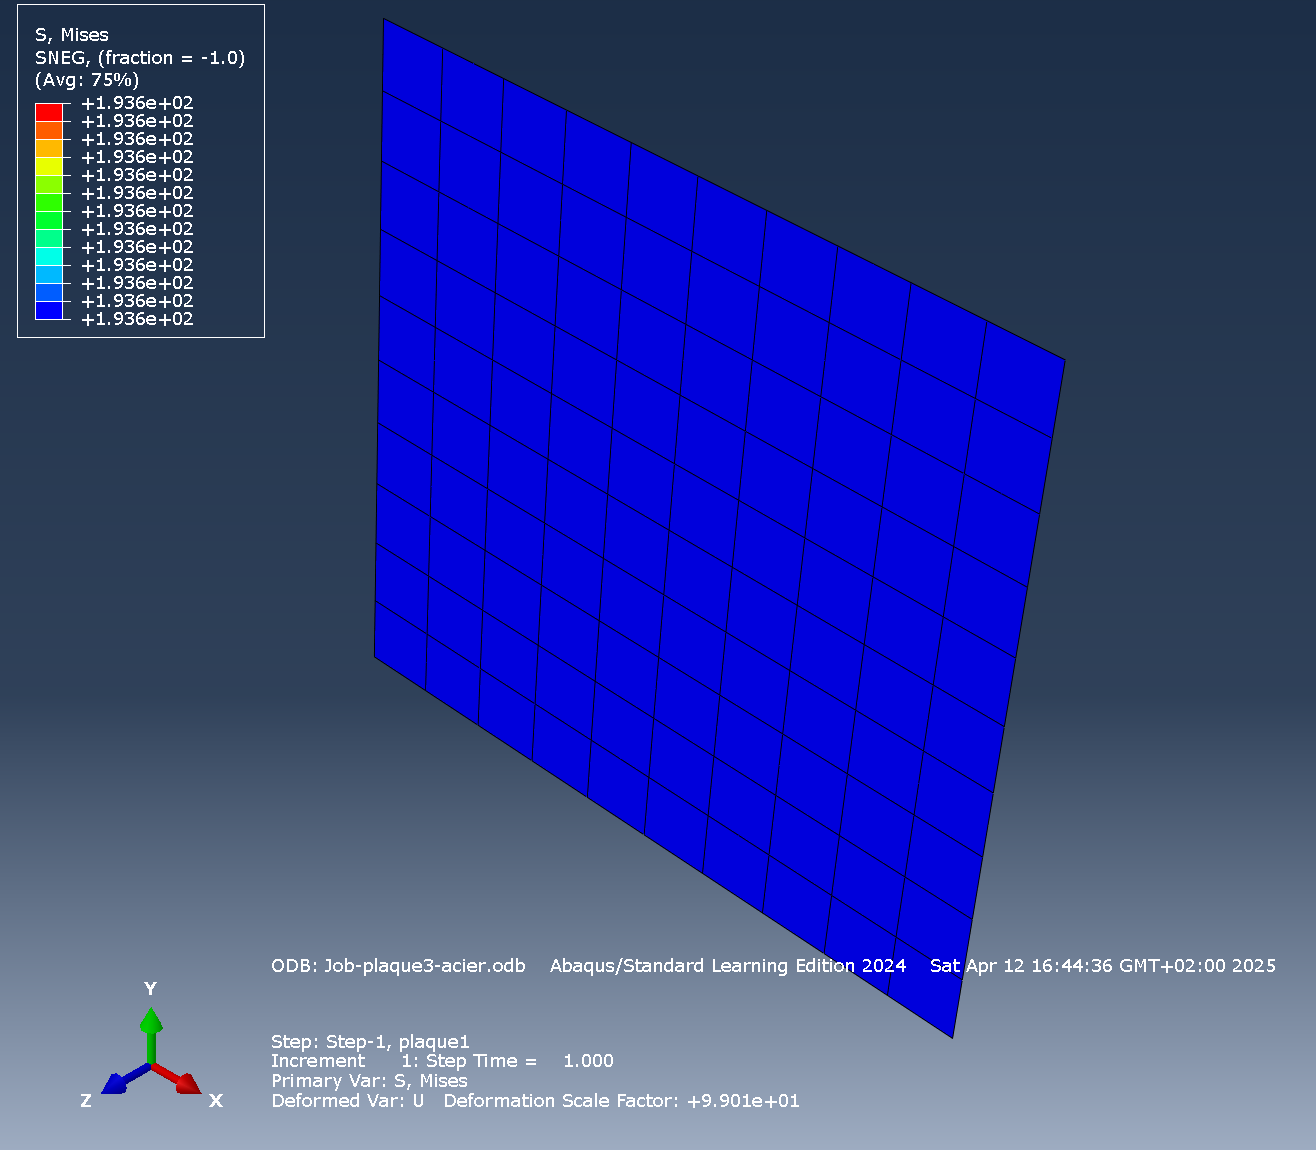
\includegraphics[width=\textwidth]{media/K_P3_mises_12042025.png} % Remplacez par le chemin de votre première image
		\caption{Plaque en acier carrée (Killian)}
		\label{fig:image1}
	\end{minipage}
	\hfill
	\begin{minipage}{0.495\textwidth}
		\centering
		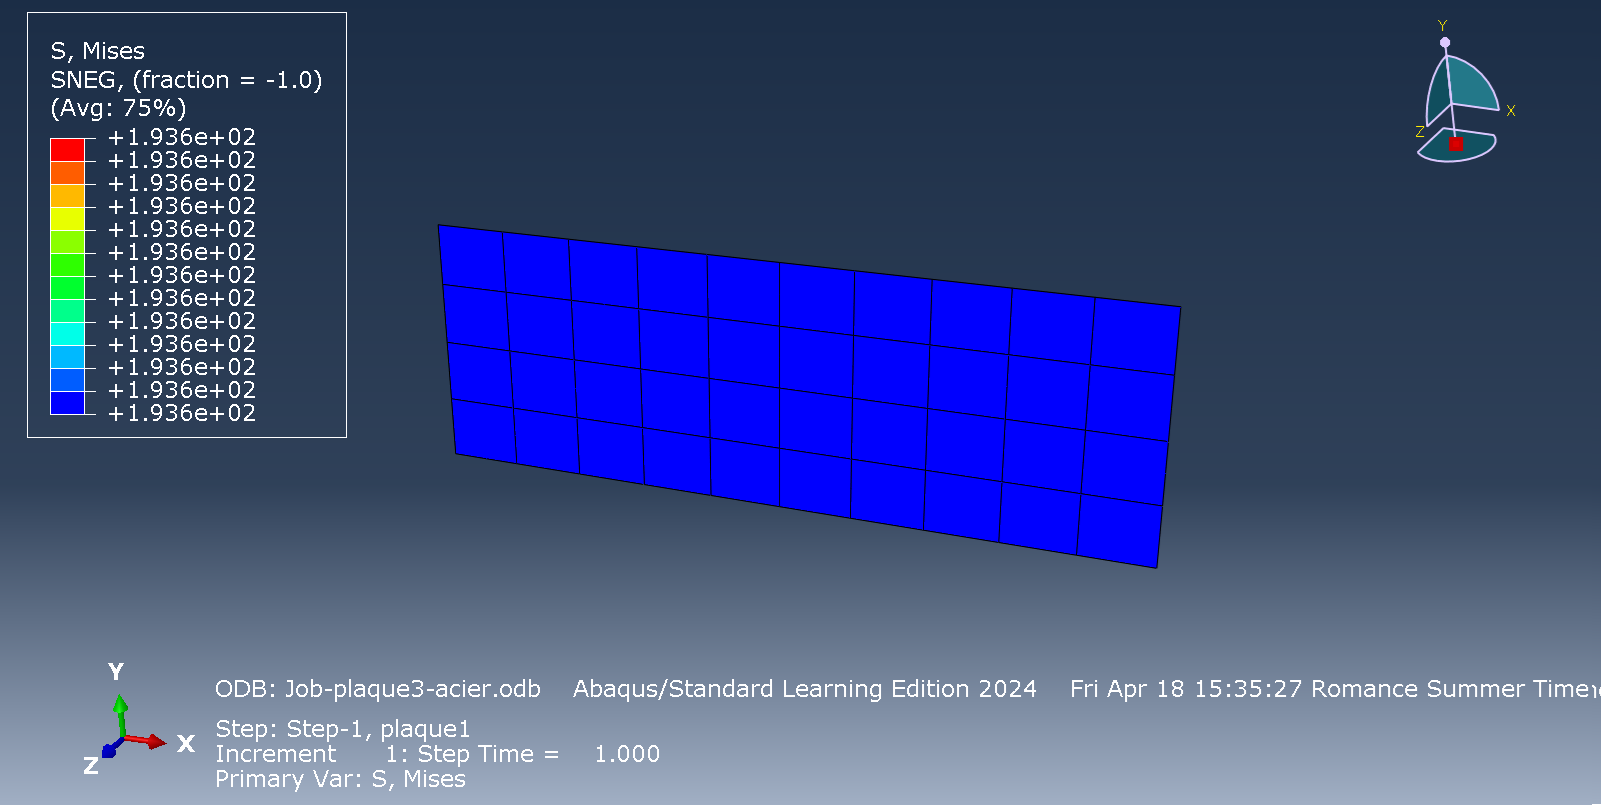
\includegraphics[width=\textwidth]{media/Plaque_metal.png} % Remplacez par le chemin de votre deuxième image
		\caption{Plaque en acier rectangle (William)}
		\label{fig:image2}
	\end{minipage}
\end{figure}

\begin{table}[H]
	\centering
	\begin{tabular}{|l|l|l|}
	\hline
	Contrainte de Von-Mises $\sigma$\textsubscript{e} & R\textsubscript{e}       & Critère \\ \hline
			194 Mpa				& 400 Mpa &     194 < 400    \\ \hline
	\end{tabular}
	\caption{Evalutation de la résistance de la plaque 3 en acier}
	\label{tab:Evalutation de la résistance de la plaque 3 en acier}
	\end{table}
La plaque en acier est donc surdimensionnée pour résister au chargement appliqué.

\subsection{Comparaison avec les résultats des autre modèles}
Nous constatons que dans cette situation (géométrie et chargement de la plaque), la plaque en acier offre de meilleures performances pour une même épaisseur que la plaque en composite. Cependant, il est important de noter que les plaques en composites sont généralement plus légères et peuvent offrir d'autres avantages en termes de résistance à la corrosion et de fatigue.

\subsection{Critique des modèles de calculs}
Les résultats obtenus sur les optimisations des paramètres du matériaux pour les plaques 1 et 2, ont été obtenus avec un programme python se basant sur le fonctionnement de la feuille de calcul. Ce programme que nous avons développé nous permet de calculer l'ensemble des critères de Tsai-Hill pour chaque combinaison de paramètres possibles. Or tester toutes les combinaison est demandant en ressource de calcul. En effet, si on considère 10 valeurs d'angle ainsi que 10 valeurs d'épaisseur, on obtient déjà plus de 100 millions de possibilités. Il a donc fallu réduire les champs possibles, ce qui fait que l'on a une précision d'environ 5° pour les angles, et de 0.5mm pour l'épaisseur de la solution optimale. Une solution à ce problème aurait pu être l'utilisaion de la méthode du simplex ou du plan d'expérience.

% Conclusion
\section{Conclusion}
Dans ce rapport, nous avons étudié trois configurations de plaques soumises à un chargement mécanique : une plaque asymétrique en composite, une plaque symétrique en composite, et une plaque en acier. Pour chaque configuration, nous avons défini les hypothèses nécessaires, mis en place un modèle numérique sous Abaqus, et comparé les résultats obtenus avec ceux calculés à l'aide d'une feuille de calcul composite.

Pour la plaque asymétrique, nous avons constaté que le critère de Tsai-Hill était dépassé, indiquant une défaillance sous le chargement appliqué. Une optimisation a été réalisée en augmentant l'épaisseur des couches, mais cela a conduit à une épaisseur totale importante, ce qui peut être un inconvénient en termes de poids et d'encombrement. Une optimisation supplémentaire basée sur l'orientation des plis a été effectuée, permettant de réduire l'épaisseur totale, tout en respectant le critère de rupture. Cela souligne l'importance de l'orientation des plis dans la conception des structures composites.

La plaque symétrique a également montré des dépassements du critère de Tsai-Hill pour certaines couches. Bien que la symétrie améliore les performances globales, des ajustements d'épaisseur ou d'orientation des plis sont nécessaires pour répondre aux exigences de résistance. On constate tout de même que la plaque symétrique se déforme moins que la plaque asymétrique, ce qui est un avantage pour la conception.
Enfin, la plaque en acier a démontré une résistance suffisante au chargement appliqué, avec une contrainte de Von Mises bien inférieure à la limite élastique. Cependant, l'acier présente d'autres inconvénients, comme une masse volumique plus élevée ($\rho_{\text{acier}} \approx 4 \cdot \rho_{\text{composite}}$) et une susceptibilité à la corrosion, ce qui peut limiter son utilisation dans certaines applications.

En conclusion, le choix du matériau pour la conception de structures dépend fortement des contraintes spécifiques de l'application. Les composites offrent des avantages en termes de légèreté et de personnalisation des propriétés mécaniques, mais nécessitent une optimisation rigoureuse pour répondre aux critères de résistance. L'acier, bien que plus lourd, reste une solution robuste et fiable pour des applications où le poids n'est pas une contrainte majeure. Une analyse multicritère intégrant les performances mécaniques, le poids, le coût et la durabilité est essentielle pour faire un choix éclairé.

\end{document}